\documentclass[]{book}
\usepackage{lmodern}
\usepackage{amssymb,amsmath}
\usepackage{ifxetex,ifluatex}
\usepackage{fixltx2e} % provides \textsubscript
\ifnum 0\ifxetex 1\fi\ifluatex 1\fi=0 % if pdftex
  \usepackage[T1]{fontenc}
  \usepackage[utf8]{inputenc}
\else % if luatex or xelatex
  \ifxetex
    \usepackage{mathspec}
  \else
    \usepackage{fontspec}
  \fi
  \defaultfontfeatures{Ligatures=TeX,Scale=MatchLowercase}
\fi
% use upquote if available, for straight quotes in verbatim environments
\IfFileExists{upquote.sty}{\usepackage{upquote}}{}
% use microtype if available
\IfFileExists{microtype.sty}{%
\usepackage{microtype}
\UseMicrotypeSet[protrusion]{basicmath} % disable protrusion for tt fonts
}{}
\usepackage[margin=1in]{geometry}
\usepackage{hyperref}
\hypersetup{unicode=true,
            pdftitle={Table of Distributions for LDA},
            pdfauthor={Jake Thornton},
            pdfborder={0 0 0},
            breaklinks=true}
\urlstyle{same}  % don't use monospace font for urls
\usepackage{natbib}
\bibliographystyle{apalike}
\usepackage{color}
\usepackage{fancyvrb}
\newcommand{\VerbBar}{|}
\newcommand{\VERB}{\Verb[commandchars=\\\{\}]}
\DefineVerbatimEnvironment{Highlighting}{Verbatim}{commandchars=\\\{\}}
% Add ',fontsize=\small' for more characters per line
\usepackage{framed}
\definecolor{shadecolor}{RGB}{248,248,248}
\newenvironment{Shaded}{\begin{snugshade}}{\end{snugshade}}
\newcommand{\KeywordTok}[1]{\textcolor[rgb]{0.13,0.29,0.53}{\textbf{#1}}}
\newcommand{\DataTypeTok}[1]{\textcolor[rgb]{0.13,0.29,0.53}{#1}}
\newcommand{\DecValTok}[1]{\textcolor[rgb]{0.00,0.00,0.81}{#1}}
\newcommand{\BaseNTok}[1]{\textcolor[rgb]{0.00,0.00,0.81}{#1}}
\newcommand{\FloatTok}[1]{\textcolor[rgb]{0.00,0.00,0.81}{#1}}
\newcommand{\ConstantTok}[1]{\textcolor[rgb]{0.00,0.00,0.00}{#1}}
\newcommand{\CharTok}[1]{\textcolor[rgb]{0.31,0.60,0.02}{#1}}
\newcommand{\SpecialCharTok}[1]{\textcolor[rgb]{0.00,0.00,0.00}{#1}}
\newcommand{\StringTok}[1]{\textcolor[rgb]{0.31,0.60,0.02}{#1}}
\newcommand{\VerbatimStringTok}[1]{\textcolor[rgb]{0.31,0.60,0.02}{#1}}
\newcommand{\SpecialStringTok}[1]{\textcolor[rgb]{0.31,0.60,0.02}{#1}}
\newcommand{\ImportTok}[1]{#1}
\newcommand{\CommentTok}[1]{\textcolor[rgb]{0.56,0.35,0.01}{\textit{#1}}}
\newcommand{\DocumentationTok}[1]{\textcolor[rgb]{0.56,0.35,0.01}{\textbf{\textit{#1}}}}
\newcommand{\AnnotationTok}[1]{\textcolor[rgb]{0.56,0.35,0.01}{\textbf{\textit{#1}}}}
\newcommand{\CommentVarTok}[1]{\textcolor[rgb]{0.56,0.35,0.01}{\textbf{\textit{#1}}}}
\newcommand{\OtherTok}[1]{\textcolor[rgb]{0.56,0.35,0.01}{#1}}
\newcommand{\FunctionTok}[1]{\textcolor[rgb]{0.00,0.00,0.00}{#1}}
\newcommand{\VariableTok}[1]{\textcolor[rgb]{0.00,0.00,0.00}{#1}}
\newcommand{\ControlFlowTok}[1]{\textcolor[rgb]{0.13,0.29,0.53}{\textbf{#1}}}
\newcommand{\OperatorTok}[1]{\textcolor[rgb]{0.81,0.36,0.00}{\textbf{#1}}}
\newcommand{\BuiltInTok}[1]{#1}
\newcommand{\ExtensionTok}[1]{#1}
\newcommand{\PreprocessorTok}[1]{\textcolor[rgb]{0.56,0.35,0.01}{\textit{#1}}}
\newcommand{\AttributeTok}[1]{\textcolor[rgb]{0.77,0.63,0.00}{#1}}
\newcommand{\RegionMarkerTok}[1]{#1}
\newcommand{\InformationTok}[1]{\textcolor[rgb]{0.56,0.35,0.01}{\textbf{\textit{#1}}}}
\newcommand{\WarningTok}[1]{\textcolor[rgb]{0.56,0.35,0.01}{\textbf{\textit{#1}}}}
\newcommand{\AlertTok}[1]{\textcolor[rgb]{0.94,0.16,0.16}{#1}}
\newcommand{\ErrorTok}[1]{\textcolor[rgb]{0.64,0.00,0.00}{\textbf{#1}}}
\newcommand{\NormalTok}[1]{#1}
\usepackage{longtable,booktabs}
\usepackage{graphicx,grffile}
\makeatletter
\def\maxwidth{\ifdim\Gin@nat@width>\linewidth\linewidth\else\Gin@nat@width\fi}
\def\maxheight{\ifdim\Gin@nat@height>\textheight\textheight\else\Gin@nat@height\fi}
\makeatother
% Scale images if necessary, so that they will not overflow the page
% margins by default, and it is still possible to overwrite the defaults
% using explicit options in \includegraphics[width, height, ...]{}
\setkeys{Gin}{width=\maxwidth,height=\maxheight,keepaspectratio}
\IfFileExists{parskip.sty}{%
\usepackage{parskip}
}{% else
\setlength{\parindent}{0pt}
\setlength{\parskip}{6pt plus 2pt minus 1pt}
}
\setlength{\emergencystretch}{3em}  % prevent overfull lines
\providecommand{\tightlist}{%
  \setlength{\itemsep}{0pt}\setlength{\parskip}{0pt}}
\setcounter{secnumdepth}{5}
% Redefines (sub)paragraphs to behave more like sections
\ifx\paragraph\undefined\else
\let\oldparagraph\paragraph
\renewcommand{\paragraph}[1]{\oldparagraph{#1}\mbox{}}
\fi
\ifx\subparagraph\undefined\else
\let\oldsubparagraph\subparagraph
\renewcommand{\subparagraph}[1]{\oldsubparagraph{#1}\mbox{}}
\fi

%%% Use protect on footnotes to avoid problems with footnotes in titles
\let\rmarkdownfootnote\footnote%
\def\footnote{\protect\rmarkdownfootnote}

%%% Change title format to be more compact
\usepackage{titling}

% Create subtitle command for use in maketitle
\newcommand{\subtitle}[1]{
  \posttitle{
    \begin{center}\large#1\end{center}
    }
}

\setlength{\droptitle}{-2em}

  \title{Table of Distributions for LDA}
    \pretitle{\vspace{\droptitle}\centering\huge}
  \posttitle{\par}
    \author{Jake Thornton}
    \preauthor{\centering\large\emph}
  \postauthor{\par}
      \predate{\centering\large\emph}
  \postdate{\par}
    \date{2019-04-26}

\usepackage{booktabs}

\begin{document}
\maketitle

{
\setcounter{tocdepth}{2}
\tableofcontents
}
\chapter*{Preface}\label{preface}
\addcontentsline{toc}{chapter}{Preface}

It is important to us that the read has accessible resources that can
support their learning when using the \emph{Loss Data Analytics} book.
\emph{Table of Distributions for LDA} aims to assist readers by
providing them with distributions used commonly throughout the book. The
distributions detailed in this resource represent all of the
distributions from the Exam C tables as well as a few other commonly
used distributions. In addition to this, each distribution has been
graphed and its corresponding density, distribution, quantile, and
random function in R.

\chapter{Continuous Distributions}\label{continuous-distributions}

\textbf{Chapter Preview}.

This table of distributions is a summary of selected continuous
probability distributions used throughout \emph{Loss Data Analytics}.

\section{Three Parameter
Distributions}\label{three-parameter-distributions}

GB2

Beta

Inv Beta

\hypertarget{3pA}{}
{Hide}

GB2

\[
{\small
\begin{matrix}
\begin{array}{l|c}
\hline
  \text{Name} & \text{Function} \\
\hline
  \text{Parameter Assumptions} & u=\Big(\frac{x}{x+\theta}\Big) \\
\hline
  \text{Probability Density Function} & \frac{\Gamma(\alpha+\tau)}{\Gamma(\alpha)\Gamma(\tau)}\frac{\theta^\alpha x^{\tau-1}}{(x+\theta)^{\alpha+\tau}} \\
    \text{f(x)} & \\
\hline
  \text{Cumulative Distribution Function} & \beta(\tau,\alpha;u) \\
    \text{F(x)} & \\
\hline
  \textit{k}^{th}~\text{Raw Moment} & \frac{\theta^k\Gamma(\tau+1)\Gamma(\alpha-k)}{\Gamma(\alpha)\Gamma(\tau)} \\
  \mathrm{E}[X^k]  & -\tau<k<\alpha \\
\hline
  \mathrm{E}[(X\wedge x)^k] & \frac{\theta^k\Gamma(\tau+k)\Gamma(\alpha-k)}{\Gamma(\alpha)\Gamma(\tau)}\beta(\tau+k,\alpha-k;u)+x^k[1-\beta(\tau,\alpha,u)]  \\
  & k>-\tau \\
\hline
\end{array}
\end{matrix}
}
\]

\begin{Shaded}
\begin{Highlighting}[]
\NormalTok{alpha=}\DecValTok{3}
\NormalTok{tau=}\DecValTok{5}
\NormalTok{theta=}\DecValTok{100}
\NormalTok{X=}\KeywordTok{seq}\NormalTok{(}\DataTypeTok{from=}\DecValTok{0}\NormalTok{,}\DataTypeTok{to=}\DecValTok{1000}\NormalTok{,}\DataTypeTok{by=}\DecValTok{1}\NormalTok{)}
\KeywordTok{plot}\NormalTok{(}\DataTypeTok{x=}\NormalTok{X,}\DataTypeTok{y=}\KeywordTok{dgenpareto}\NormalTok{(X,}\DataTypeTok{shape1=}\NormalTok{alpha,}\DataTypeTok{shape2=}\NormalTok{tau,}\DataTypeTok{scale=}\NormalTok{theta),}\DataTypeTok{type=}\StringTok{"l"}\NormalTok{,}\DataTypeTok{ylab=}\StringTok{"Probability density"}\NormalTok{,}\DataTypeTok{col=}\StringTok{"red"}\NormalTok{,}\DataTypeTok{main=}\StringTok{"GB2 Distribution"}\NormalTok{)}
\end{Highlighting}
\end{Shaded}

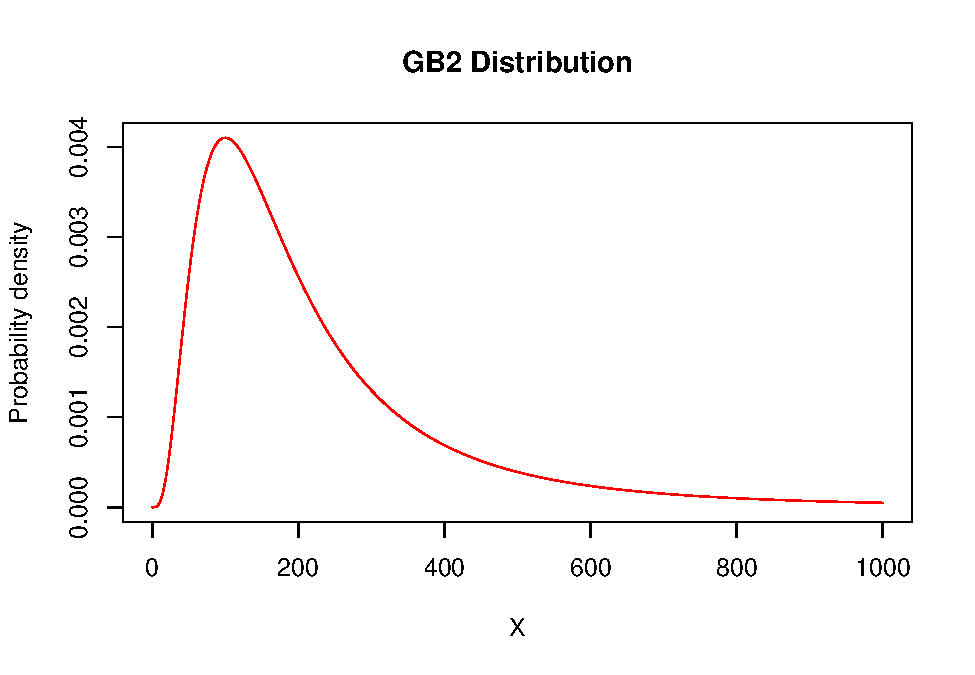
\includegraphics{LDASupplements_files/figure-latex/unnamed-chunk-2-1.pdf}

\[
{\small
\begin{matrix}
\begin{array}{l|c}
\hline
  \text{Density Function} & \text{dgenpareto}(x=, shape1=\alpha, shape2=\tau, scale=\theta) \\
\hline
  \text{Distribution Function} & \text{pgenpareto}(q=, shape1=\alpha, shape2=\tau, scale=\theta) \\
\hline
  \text{Quantile Function} & \text{qgenpareto}(p=, shape1=\alpha, shape2=\tau, scale=\theta) \\ 
\hline
  \text{Random Sampling Function} & \text{rgenpareto}(r=, shape1=\alpha, shape2=\tau, scale=\theta) \\
\hline
\end{array}
\end{matrix}
}
\]

\hypertarget{3pB}{}
{Hide}

Burr

\[
{\small
\begin{matrix}
\begin{array}{l|c}
\hline
  \text{Name} & \text{Function} \\
\hline
  \text{Parameter Assumptions} & u=\frac{1}{1+(x/\theta)^\gamma} \\
\hline
  \text{Probability Density Function} & \frac{\alpha\gamma(x/\theta)^\gamma}{x[1+(x/\theta)^\gamma]^{\alpha+1}} \\
    \text{f(x)} & \\
\hline
  \text{Cumulative Distribution Function} & 1-u^\alpha \\
    \text{F(x)} & \\
\hline
  \textit{k}^{th}~\text{Raw Moment} & \frac{\theta\Gamma(1+(k/\gamma))\Gamma(\alpha-(k/\gamma))}{\Gamma(\alpha)} \\
  \mathrm{E}[X^k]  & -\gamma<k<\alpha\gamma \\
\hline
  \mathrm{E}[(X\wedge x)^k] & \frac{\theta\Gamma(1+(k/\gamma))\Gamma(\alpha-(k/\gamma))}{\Gamma(\alpha)}\beta(1+(k/\gamma),\alpha-(k/\gamma);1-u)+x^ku^\alpha  \\
  & k>-\tau \\
\hline
\end{array}
\end{matrix}
}
\]

\begin{Shaded}
\begin{Highlighting}[]
\NormalTok{alpha=}\DecValTok{2}
\NormalTok{gamma=}\DecValTok{3}
\NormalTok{theta=}\DecValTok{100}
\NormalTok{X=}\KeywordTok{seq}\NormalTok{(}\DataTypeTok{from=}\DecValTok{0}\NormalTok{,}\DataTypeTok{to=}\DecValTok{1000}\NormalTok{,}\DataTypeTok{by=}\DecValTok{1}\NormalTok{)}
\KeywordTok{plot}\NormalTok{(}\DataTypeTok{x=}\NormalTok{X,}\DataTypeTok{y=}\KeywordTok{dburr}\NormalTok{(X,}\DataTypeTok{shape1=}\NormalTok{alpha,}\DataTypeTok{shape2=}\NormalTok{gamma,}\DataTypeTok{scale=}\NormalTok{theta),}\DataTypeTok{type=}\StringTok{"l"}\NormalTok{,}\DataTypeTok{ylab=}\StringTok{"Probability density"}\NormalTok{,}\DataTypeTok{col=}\StringTok{"red"}\NormalTok{,}\DataTypeTok{main=}\StringTok{"Burr Distribution"}\NormalTok{)}
\end{Highlighting}
\end{Shaded}

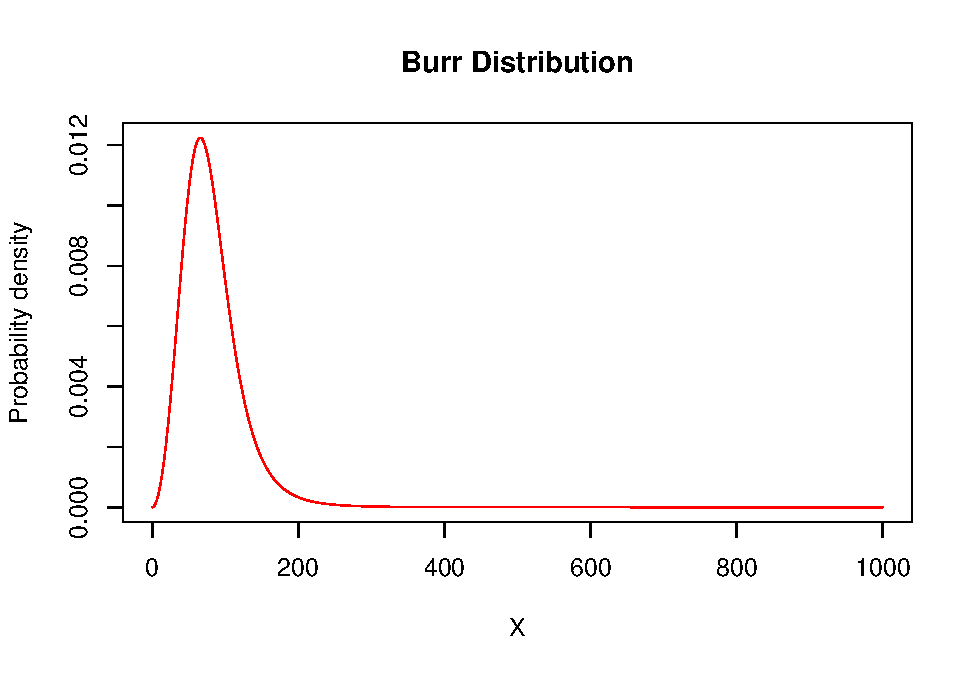
\includegraphics{LDASupplements_files/figure-latex/unnamed-chunk-3-1.pdf}

\[
{\small
\begin{matrix}
\begin{array}{l|c}
\hline
  \text{Density Function} & \text{dburr}(x=, shape1=\alpha, shape2=\gamma, scale=\theta) \\
\hline
  \text{Distribution Function} & \text{pburr}(p=, shape1=\alpha, shape2=\gamma, scale=\theta) \\
\hline
  \text{Quantile Function} & \text{qburr}(q=, shape1=\alpha, shape2=\gamma, scale=\theta) \\ 
\hline
  \text{Random Sampling Function} & \text{rburr}(n=, shape1=\alpha, shape2=\gamma, scale=\theta) \\
\hline
\end{array}
\end{matrix}
}
\]

\hypertarget{3pC}{}
{Hide}

Inv Burr

\[
{\small
\begin{matrix}
\begin{array}{l|c}
\hline
  \text{Name} & \text{Function} \\
\hline
  \text{Parameter Assumptions} & u=\frac{(x/\theta)^\gamma}{1+(x/\theta)^\gamma} \\
\hline
  \text{Probability Density Function} & \frac{\alpha\gamma(x/\theta)^\gamma}{x[1+(x/\theta)^\tau]^{\alpha+1}} \\
    \text{f(x)} & \\
\hline
  \text{Cumulative Distribution Function} & u^\tau \\
    \text{F(x)} & \\
\hline
  \textit{k}^{th}~\text{Raw Moment} & \frac{\theta^k\Gamma(1+(k/\gamma))\Gamma(\alpha-(k/\gamma))}{\tau} \\
  \mathrm{E}[X^k]  & -\tau\gamma<k<\gamma \\
\hline
  \mathrm{E}[(X\wedge x)^k] & \frac{\theta^k\Gamma(1+(k/\gamma))\Gamma(\alpha-(k/\gamma))}{\tau}\beta(\tau+(k/\gamma),1-(k/\gamma);u)+x^k[1-u^\tau]  \\
  & k>-\tau \\
\hline
\end{array}
\end{matrix}
}
\]

\begin{Shaded}
\begin{Highlighting}[]
\NormalTok{alpha=}\DecValTok{2}
\NormalTok{tau=}\DecValTok{3}
\NormalTok{theta=}\DecValTok{100}
\NormalTok{X=}\KeywordTok{seq}\NormalTok{(}\DataTypeTok{from=}\DecValTok{0}\NormalTok{,}\DataTypeTok{to=}\DecValTok{1000}\NormalTok{,}\DataTypeTok{by=}\DecValTok{1}\NormalTok{)}
\KeywordTok{plot}\NormalTok{(}\DataTypeTok{x=}\NormalTok{X,}\DataTypeTok{y=}\KeywordTok{dinvburr}\NormalTok{(X,}\DataTypeTok{shape1=}\NormalTok{alpha,}\DataTypeTok{shape2=}\NormalTok{tau,}\DataTypeTok{scale=}\NormalTok{theta),}\DataTypeTok{type=}\StringTok{"l"}\NormalTok{,}\DataTypeTok{ylab=}\StringTok{"Probability density"}\NormalTok{,}\DataTypeTok{col=}\StringTok{"red"}\NormalTok{,}\DataTypeTok{main=}\StringTok{"Inv Burr Distribution"}\NormalTok{)}
\end{Highlighting}
\end{Shaded}

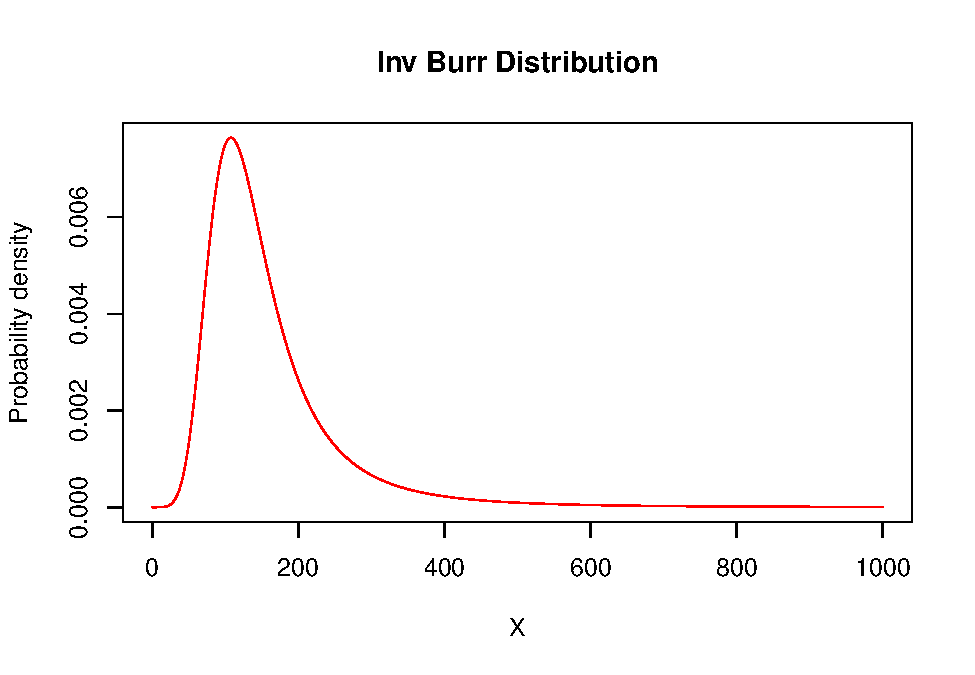
\includegraphics{LDASupplements_files/figure-latex/unnamed-chunk-4-1.pdf}

\[
{\small
\begin{matrix}
\begin{array}{l|c}
\hline
  \text{Density Function} & \text{dinvburr}(x=, shape1=\alpha, shape2=\tau, scale=\theta) \\
\hline
  \text{Distribution Function} & \text{pinvburr}(p=, shape1=\alpha, shape2=\tau, scale=\theta) \\
\hline
  \text{Quantile Function} & \text{qinvburr}(q=, shape1=\alpha, shape2=\tau, scale=\theta) \\ 
\hline
  \text{Random Sampling Function} & \text{rinvburr}(n=, shape1=\alpha, shape2=\tau, scale=\theta) \\
\hline
\end{array}
\end{matrix}
}
\]

\section{Two Parameter Distributions}\label{two-parameter-distributions}

Pareto

Inv Pareto

Loglogistic

Paralogistic

Gamma

Inv Gamma

Weibull

Inv Weibull

\hypertarget{2pA}{}
{Hide}

Pareto

\[
{\small
\begin{matrix}
\begin{array}{l|c}
\hline
  \text{Name} & \text{Function} \\
\hline
  \text{Parameter Assumptions} & \alpha>0 \\
\hline
  \text{Probability Density Function} & \frac{\alpha\theta^\alpha}{(x+\theta)^{\alpha+1}} \\
    \text{f(x)} & \\
\hline
  \text{Cumulative Distribution Function} & 1-\Big(\frac{\theta}{x+\theta}\Big)^\alpha \\
    \text{F(x)} & \\
\hline
  \textit{k}^{th}~\text{Raw Moment} & \frac{\theta^k\Gamma(k+1)\Gamma(\alpha-k)}{\Gamma(\alpha)} \\
  \mathrm{E}[X^k] & -1<\alpha<k \\
\hline
  \text{Limited Expected Value:}~\alpha\neq1 & \frac{\theta}{\alpha-1}\Big[1-\Big(\frac{\theta}{x+\theta}\Big)^{\alpha-1}\Big] \\
  \mathrm{E}[X\wedge x] & \\
\hline
  \text{Limited Expected Value:}~\alpha=1 & -\theta ln\left(\frac{\theta}{x+\theta}\right) \\
  \mathrm{E}[X\wedge x] & \\
\hline
  \mathrm{E}[(X\wedge x)^k] & \frac{\theta^k\Gamma(k+1)\Gamma(\alpha-k)}{\Gamma(\alpha)}\beta(k+1,\alpha-k;\frac{x}{x+\theta})+x^k(\frac{\theta}{x+\theta})^\alpha  \\
\hline
\end{array}
\end{matrix}
}
\]

\begin{Shaded}
\begin{Highlighting}[]
\NormalTok{alpha=}\DecValTok{3}
\NormalTok{theta=}\DecValTok{200}
\NormalTok{X=}\KeywordTok{seq}\NormalTok{(}\DataTypeTok{from=}\DecValTok{0}\NormalTok{,}\DataTypeTok{to=}\DecValTok{1000}\NormalTok{,}\DataTypeTok{by=}\DecValTok{1}\NormalTok{)}
\KeywordTok{plot}\NormalTok{(}\DataTypeTok{x=}\NormalTok{X,}\DataTypeTok{y=}\KeywordTok{dpareto2}\NormalTok{(X,}\DataTypeTok{shape=}\NormalTok{alpha,}\DataTypeTok{scale=}\NormalTok{theta),}\DataTypeTok{type=}\StringTok{"l"}\NormalTok{,}\DataTypeTok{ylab=}\StringTok{"Probability density"}\NormalTok{,}\DataTypeTok{col=}\StringTok{"red"}\NormalTok{,}\DataTypeTok{main=}\StringTok{"Pareto Distribution"}\NormalTok{)}
\end{Highlighting}
\end{Shaded}

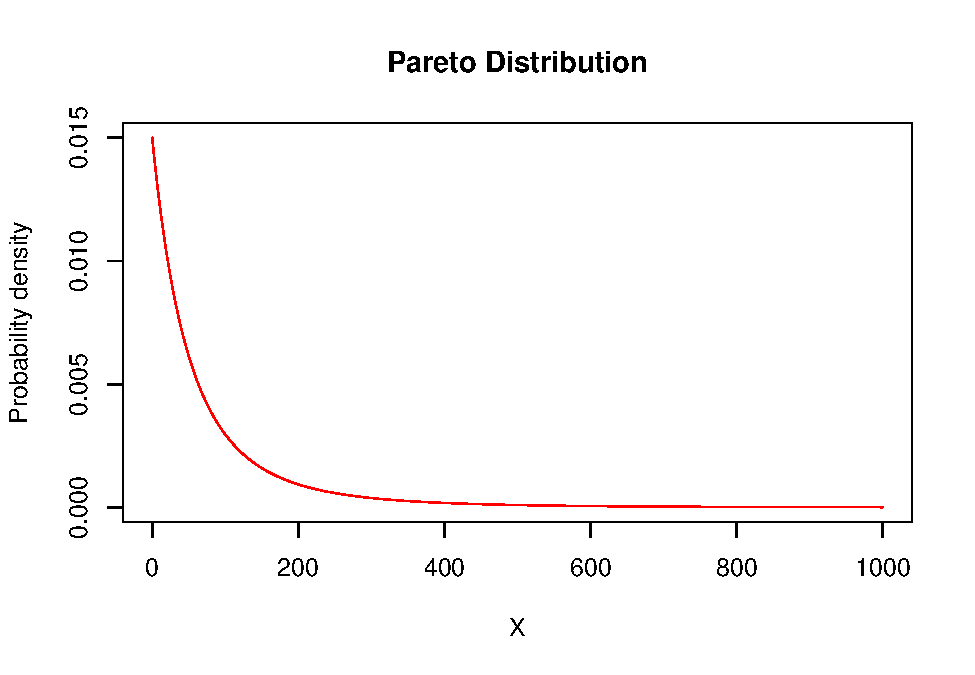
\includegraphics{LDASupplements_files/figure-latex/unnamed-chunk-5-1.pdf}

\[
{\small
\begin{matrix}
\begin{array}{l|c}
\hline
  \text{Density Function} & \text{dpareto2}(x=, shape=\alpha, scale=\theta) \\
\hline
  \text{Distribution Function} & \text{ppareto2}(p=, shape=\alpha,scale=\theta) \\
\hline
  \text{Quantile Function} & \text{qpareto2}(q=, shape=\alpha,scale=\theta) \\ 
\hline
  \text{Random Sampling Function} & \text{rpareto2}(n=, shape=\alpha,scale=\theta) \\
\hline
\end{array}
\end{matrix}
}
\]

\hypertarget{2pB}{}
{Hide}

Inv Pareto

\[
{\small
\begin{matrix}
\begin{array}{l|c}
\hline
  \text{Name} & \text{Function} \\
\hline
  \text{Probability Density Function} & \frac{\tau\theta x^{\tau-1}}{(x+\theta)^\tau-1} \\
    \text{f(x)} & \\
\hline
  \text{Cumulative Distribution Function} & \Big(\frac{x}{x+\theta}\Big)^\tau \\
    \text{F(x)} & \\
\hline
  \textit{k}^{th}~\text{Raw Moment} & \frac{\theta^k\Gamma(\tau+k)\Gamma(1-k)}{\Gamma(\tau)} \\
  \mathrm{E}[X^k]  & -\tau<k<1 \\
\hline
  \mathrm{E}[(X\wedge x)^k] & \theta^k\tau\int^{x/(x+\theta)}_0~y^{\tau+k-1}(1-y)^{-k}dy+x^k[1-\Big(\frac{x}{x+\theta}\Big)^\tau] \\
  & k>-\tau \\
\hline
\end{array}
\end{matrix}
}
\]

\begin{Shaded}
\begin{Highlighting}[]
\NormalTok{tau=}\DecValTok{5}
\NormalTok{theta=}\DecValTok{100}
\NormalTok{X=}\KeywordTok{seq}\NormalTok{(}\DataTypeTok{from=}\DecValTok{0}\NormalTok{,}\DataTypeTok{to=}\DecValTok{3000}\NormalTok{,}\DataTypeTok{by=}\DecValTok{1}\NormalTok{)}
\KeywordTok{plot}\NormalTok{(}\DataTypeTok{x=}\NormalTok{X,}\DataTypeTok{y=}\KeywordTok{dinvpareto}\NormalTok{(X,}\DataTypeTok{shape=}\NormalTok{tau,}\DataTypeTok{scale=}\NormalTok{theta),}\DataTypeTok{type=}\StringTok{"l"}\NormalTok{,}\DataTypeTok{ylab=}\StringTok{"Probability density"}\NormalTok{,}\DataTypeTok{col=}\StringTok{"red"}\NormalTok{,}\DataTypeTok{main=}\StringTok{"Inv Pareto Distribution"}\NormalTok{)}
\end{Highlighting}
\end{Shaded}

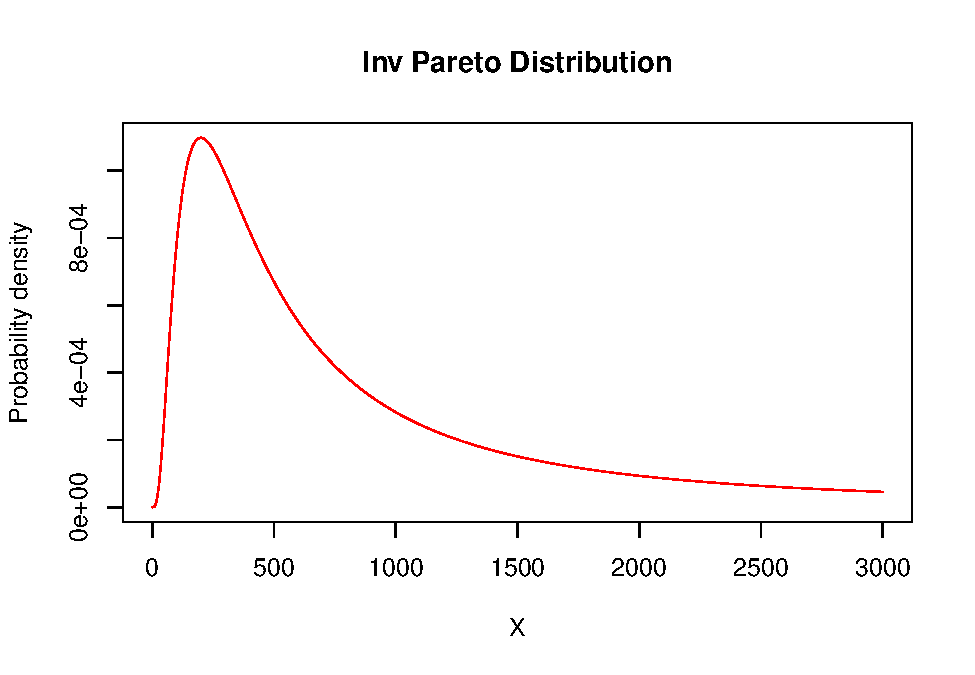
\includegraphics{LDASupplements_files/figure-latex/unnamed-chunk-6-1.pdf}

\[
{\small
\begin{matrix}
\begin{array}{l|c}
\hline
  \text{Density Function} & \text{dinvpareto}(x=, shape=\tau, scale=\theta) \\
\hline
  \text{Distribution Function} & \text{pinvpareto}(p=, shape=\tau,scale=\theta) \\
\hline
  \text{Quantile Function} & \text{qinvpareto}(q=, shape=\tau,scale=\theta) \\ 
\hline
  \text{Random Sampling Function} & \text{rinvpareto}(n=, shape=\tau,scale=\theta) \\
\hline
\end{array}
\end{matrix}
}
\]

\hypertarget{2pC}{}
{Hide}

Loglogistic

\[
{\small
\begin{matrix}
\begin{array}{l|c}
\hline
  \text{Name} & \text{Function} \\
\hline
  \text{Parameter Assumptions} & u=\frac{(x/\theta)^\gamma}{1+(x/\theta)^\gamma} \\
\hline
  \text{Probability Density Function} & \frac{\gamma(x/\theta)^\gamma}{x[1+(x/\theta)^\gamma]^2} \\
    \text{f(x)} & \\
\hline
  \text{Cumulative Distribution Function} & u \\
    \text{F(x)} & \\
\hline
  \textit{k}^{th}~\text{Raw Moment} & \theta^k\Gamma(1+(k/\gamma))\Gamma(1-(k/\gamma)) \\
  \mathrm{E}[X^k]  & -\gamma<k<\gamma \\
\hline
  \mathrm{E}[(X\wedge x)^k] & \theta^k\Gamma(1+(k/\gamma))\Gamma(1-(k/\gamma))\beta(1+(k/\gamma),1-(k/\gamma);u)+x^k(1-u) \\
  & k>-\gamma \\
\hline
\end{array}
\end{matrix}
}
\]

\begin{Shaded}
\begin{Highlighting}[]
\CommentTok{#need to write a f(x) for this dist}
\end{Highlighting}
\end{Shaded}

\hypertarget{2pD}{}
{Hide}

Paralogistic

\[
{\small
\begin{matrix}
\begin{array}{l|c}
\hline
  \text{Name} & \text{Function} \\
\hline
  \text{Parameter Assumptions} & u=\frac{1}{1+(x/\theta)^\alpha} \\
\hline
  \text{Probability Density Function} & \frac{\alpha^2(x/\theta)^\alpha}{x[1+(x/\theta)^\alpha]^{\alpha+1}} \\
    \text{f(x)} & \\
\hline
  \text{Cumulative Distribution Function} & 1-u^\alpha \\
    \text{F(x)} & \\
\hline
  \textit{k}^{th}~\text{Raw Moment} & \frac{\theta^k\Gamma(1+(k/\alpha))\Gamma(\alpha-(k/\alpha))}{\Gamma(\alpha)} \\
  \mathrm{E}[X^k]  & -\alpha<k<\alpha^2 \\
\hline
  \mathrm{E}[(X\wedge x)^k] & \frac{\theta^k\Gamma(1+(k/\alpha))\Gamma(\alpha-(k/\alpha))}{\Gamma(\alpha)}\beta(1+(k/\alpha),\alpha-(k/\alpha);1-u)+x^\alpha \\
  & k>-\alpha \\
\hline
\end{array}
\end{matrix}
}
\]

\begin{Shaded}
\begin{Highlighting}[]
\NormalTok{alpha=}\DecValTok{2}
\NormalTok{theta=}\DecValTok{100}
\NormalTok{X=}\KeywordTok{seq}\NormalTok{(}\DataTypeTok{from=}\DecValTok{0}\NormalTok{,}\DataTypeTok{to=}\DecValTok{1000}\NormalTok{,}\DataTypeTok{by=}\DecValTok{1}\NormalTok{)}
\KeywordTok{plot}\NormalTok{(}\DataTypeTok{x=}\NormalTok{X,}\DataTypeTok{y=}\KeywordTok{dparalogis}\NormalTok{(X,}\DataTypeTok{shape=}\NormalTok{alpha,}\DataTypeTok{scale=}\NormalTok{theta),}\DataTypeTok{type=}\StringTok{"l"}\NormalTok{,}\DataTypeTok{ylab=}\StringTok{"Probability density"}\NormalTok{,}\DataTypeTok{col=}\StringTok{"red"}\NormalTok{,}\DataTypeTok{main=}\StringTok{"Paralogistic Distribution"}\NormalTok{)}
\end{Highlighting}
\end{Shaded}

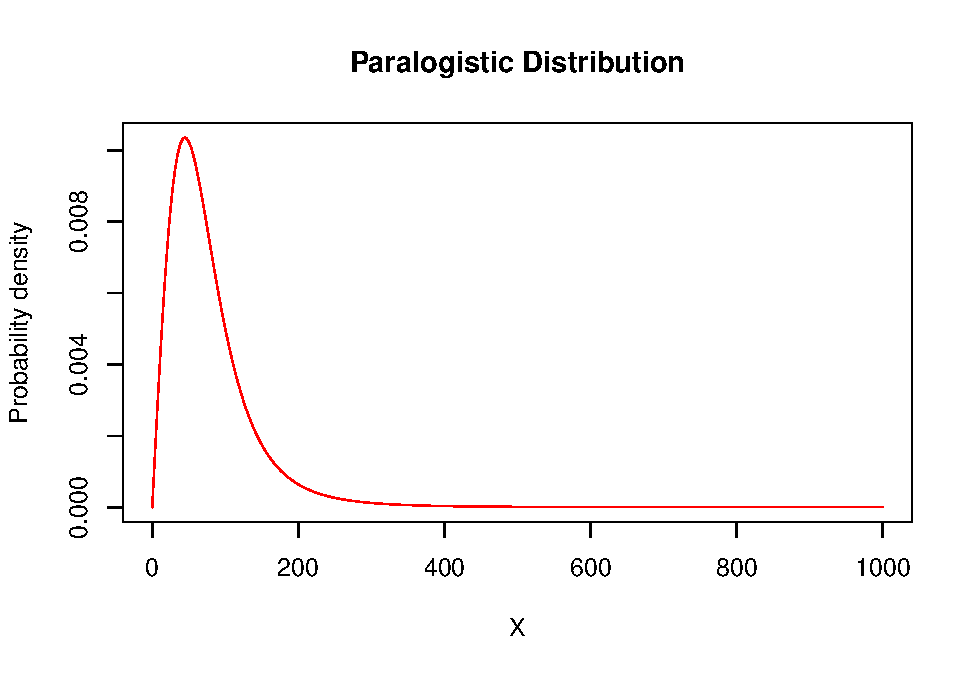
\includegraphics{LDASupplements_files/figure-latex/unnamed-chunk-8-1.pdf}

\[
{\small
\begin{matrix}
\begin{array}{l|c}
\hline
  \text{Density Function} & \text{dparalogis}(x=, shape=\alpha, scale=\theta) \\
\hline
  \text{Distribution Function} & \text{pparalogis}(p=, shape=\alpha,scale=\theta) \\
\hline
  \text{Quantile Function} & \text{qparalogis}(q=, shape=\alpha,scale=\theta) \\ 
\hline
  \text{Random Sampling Function} & \text{rparalogis}(n=, shape=\alpha,scale=\theta) \\
\hline
\end{array}
\end{matrix}
}
\]

\hypertarget{2pE}{}
{Hide}

Gamma

\[
{\small
\begin{matrix}
\begin{array}{l|c}
\hline
  \text{Name} & \text{Function} \\
\hline
  \text{Parameter Assumptions} & \theta>0,~\alpha>0 \\
\hline
  \text{Probability Density Function} & \frac{1}{\theta^{\alpha}\Gamma(\alpha)}x^{\alpha-1}e^{-x/\theta} \\
    \text{f(x)} & \\
\hline
  \text{Cumulative Distribution Function} & \Gamma(\alpha;\frac{x}{\theta}) \\
    \text{F(x)} & \\
\hline
  \textit{k}^{th}~\text{Raw Moment}  & \theta^k\frac{\Gamma(\alpha+k)}{\Gamma(\alpha)} \\
  \mathrm{E}[X^k]  & k>-\alpha \\
\hline
  \text{Limited Expected Value} & \frac{\theta^k\Gamma(k+\alpha)}{\Gamma(\alpha)}\Gamma(k+\alpha; x/\theta)+x^k[1-\Gamma(\alpha; x/\theta)]  \\
   \mathrm{E}[X\wedge x] & k > -\alpha \\
\hline
\end{array}
\end{matrix}
}
\]

\begin{Shaded}
\begin{Highlighting}[]
\NormalTok{alpha=}\DecValTok{2}
\NormalTok{theta=}\DecValTok{50}
\NormalTok{X=}\KeywordTok{seq}\NormalTok{(}\DataTypeTok{from=}\DecValTok{0}\NormalTok{,}\DataTypeTok{to=}\DecValTok{1000}\NormalTok{,}\DataTypeTok{by=}\DecValTok{1}\NormalTok{)}
\KeywordTok{plot}\NormalTok{(}\DataTypeTok{x=}\NormalTok{X,}\DataTypeTok{y=}\KeywordTok{dgamma}\NormalTok{(X,}\DataTypeTok{shape=}\NormalTok{alpha,}\DataTypeTok{scale=}\NormalTok{theta),}\DataTypeTok{type=}\StringTok{"l"}\NormalTok{,}\DataTypeTok{ylab=}\StringTok{"Probability density"}\NormalTok{,}\DataTypeTok{col=}\StringTok{"red"}\NormalTok{,}\DataTypeTok{main=}\StringTok{"Gamma Distribution"}\NormalTok{)}
\end{Highlighting}
\end{Shaded}

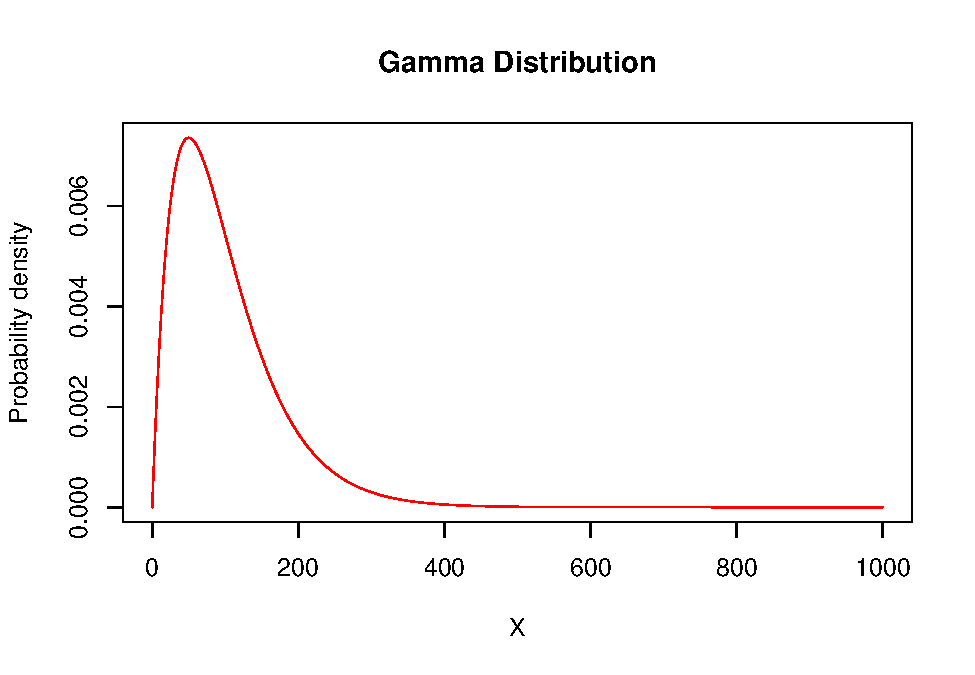
\includegraphics{LDASupplements_files/figure-latex/unnamed-chunk-9-1.pdf}

\[
{\small
\begin{matrix}
\begin{array}{l|c}
\hline
  \text{Density Function} & \text{dgamma}(x=, shape=\alpha, scale=\theta) \\
\hline
  \text{Distribution Function} & \text{pgamma}(p=, shape=\alpha,scale=\theta) \\
\hline
  \text{Quantile Function} & \text{qgamma}(q=, shape=\alpha,scale=\theta) \\ 
\hline
  \text{Random Sampling Function} & \text{rgamma}(n=, shape=\alpha,scale=\theta) \\
\hline
\end{array}
\end{matrix}
}
\]

\hypertarget{2pF}{}
{Hide}

Inv Gamma

\[
{\small
\begin{matrix}
\begin{array}{l|c}
\hline
  \text{Name} & \text{Function} \\
\hline
  \text{Probability Density Function} & \frac{(\theta/x)^\alpha e^{-\theta/x}}{x\Gamma(\alpha)} \\
    \text{f(x)} & \\
\hline
  \text{Cumulative Distribution Function} & 1-\Gamma(\alpha;\theta/x) \\
    \text{F(x)} & \\
\hline
  \textit{k}^{th}~\text{Raw Moment} & \frac{\theta^k\Gamma(\alpha-k)}{\Gamma(\alpha)} \\
  \mathrm{E}[X^k]  & k<\alpha \\
\hline
  \mathrm{E}[(X\wedge x)^k] & \frac{\theta^k\Gamma(\alpha-k)}{\Gamma(\alpha)}[1-\Gamma(\alpha-k;\theta/x)]+x^k\Gamma(\alpha;\theta/x) \\
  &  \\
\hline
\end{array}
\end{matrix}
}
\]

\begin{Shaded}
\begin{Highlighting}[]
\NormalTok{alpha=}\DecValTok{3}
\NormalTok{theta=}\DecValTok{100}
\NormalTok{X=}\KeywordTok{seq}\NormalTok{(}\DataTypeTok{from=}\DecValTok{0}\NormalTok{,}\DataTypeTok{to=}\DecValTok{400}\NormalTok{,}\DataTypeTok{by=}\DecValTok{1}\NormalTok{)}
\KeywordTok{plot}\NormalTok{(}\DataTypeTok{x=}\NormalTok{X,}\DataTypeTok{y=}\KeywordTok{dinvgamma}\NormalTok{(X,}\DataTypeTok{shape=}\NormalTok{alpha,}\DataTypeTok{scale=}\NormalTok{theta),}\DataTypeTok{type=}\StringTok{"l"}\NormalTok{,}\DataTypeTok{ylab=}\StringTok{"Probability density"}\NormalTok{,}\DataTypeTok{col=}\StringTok{"red"}\NormalTok{,}\DataTypeTok{main=}\StringTok{"Inv Gamma Distribution"}\NormalTok{)}
\end{Highlighting}
\end{Shaded}

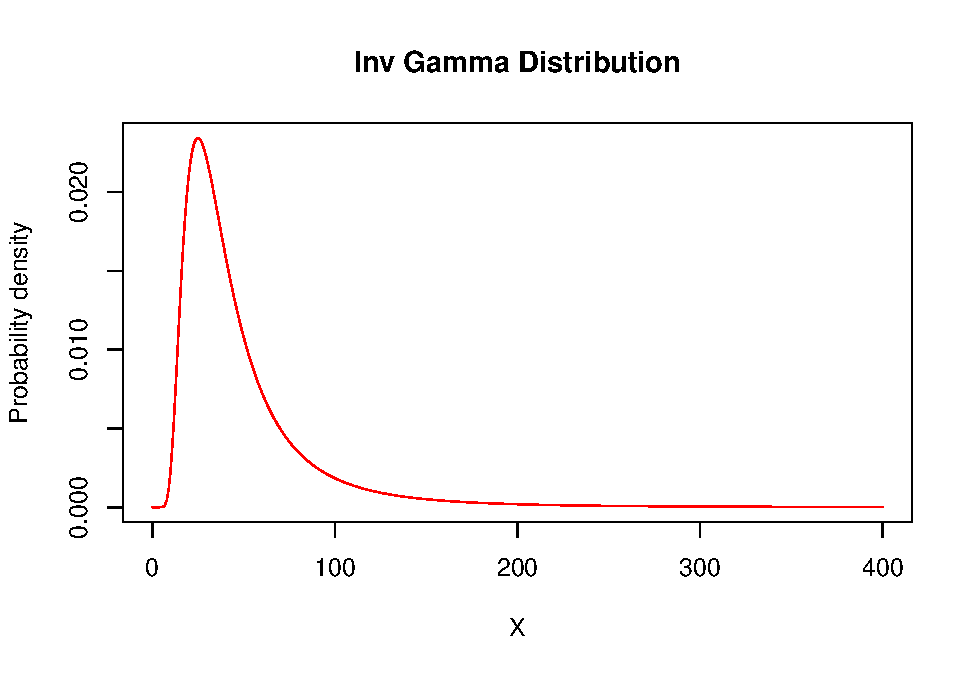
\includegraphics{LDASupplements_files/figure-latex/unnamed-chunk-10-1.pdf}

\[
{\small
\begin{matrix}
\begin{array}{l|c}
\hline
  \text{Density Function} & \text{dinvgamma}(x=, shape=\alpha, scale=\theta) \\
\hline
  \text{Distribution Function} & \text{pinvgamma}(p=, shape=\alpha,scale=\theta) \\
\hline
  \text{Quantile Function} & \text{qinvgamma}(q=, shape=\alpha,scale=\theta) \\ 
\hline
  \text{Random Sampling Function} & \text{rinvgamma}(n=, shape=\alpha,scale=\theta) \\
\hline
\end{array}
\end{matrix}
}
\]

\hypertarget{2pG}{}
{Hide}

Weibull

\[
{\small
\begin{matrix}
\begin{array}{l|c}
\hline
  \text{Name} & \text{Function} \\
\hline
  \text{Parameter Assumptions} &  \\
\hline\
  \text{Probability Density Function} & \frac{\tau \Big(\frac{\theta}{x}\Big)^\tau e^-\Big(\frac{\theta}{x}\Big)^\tau}{x} \\
    \text{f(x)} & \\
\hline
  \text{Cumulative Distribution Function} & \exp\Big(-\Big(\frac{\theta}{x}\Big)^\tau\Big) \\
    \text{F(x)} & \\
\hline
  \textit{k}^{th}~\text{Raw Moment} & \theta^k \Gamma(1 + \frac{k}{\tau}) \\
  \mathrm{E}[X^k]  & k>-\tau \\
\hline
  \mathrm{E}[(X\wedge x)^k] & \theta^k\Gamma(1+\frac{k}{\tau})\Gamma\Big[1+\frac{k}{\tau};\Big(\frac{x}{\theta}\Big)^\tau\Big]+x^k\exp\Big(-\Big(\frac{x}{\tau}\Big)^\tau\Big)  \\
   & k>-\tau \\
\hline
\end{array}
\end{matrix}
}
\]

\begin{Shaded}
\begin{Highlighting}[]
\NormalTok{tau=}\DecValTok{2}
\NormalTok{theta=}\DecValTok{100}
\NormalTok{X=}\KeywordTok{seq}\NormalTok{(}\DataTypeTok{from=}\DecValTok{0}\NormalTok{,}\DataTypeTok{to=}\DecValTok{1000}\NormalTok{,}\DataTypeTok{by=}\DecValTok{1}\NormalTok{)}
\KeywordTok{plot}\NormalTok{(}\DataTypeTok{x=}\NormalTok{X,}\DataTypeTok{y=}\KeywordTok{dweibull}\NormalTok{(X,}\DataTypeTok{shape=}\NormalTok{tau, }\DataTypeTok{scale=}\NormalTok{theta),}\DataTypeTok{type=}\StringTok{"l"}\NormalTok{,}\DataTypeTok{ylab=}\StringTok{"Probability density"}\NormalTok{,}\DataTypeTok{col=}\StringTok{"red"}\NormalTok{,}\DataTypeTok{main=}\StringTok{"Weibull Distribution"}\NormalTok{)}
\end{Highlighting}
\end{Shaded}

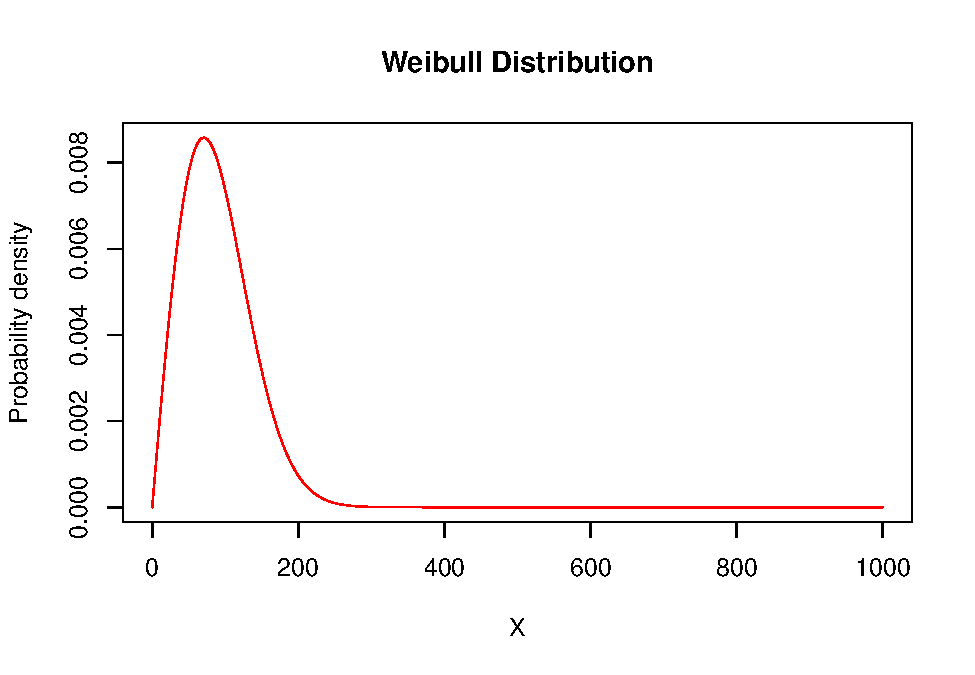
\includegraphics{LDASupplements_files/figure-latex/unnamed-chunk-11-1.pdf}

\[
{\small
\begin{matrix}
\begin{array}{l|c}
\hline
  \text{Density Function} & \text{dweibull}(x=, shape=\tau, scale=\theta) \\
\hline
  \text{Distribution Function} & \text{pweibull}(p=, shape=\tau,scale=\theta) \\
\hline
  \text{Quantile Function} & \text{qweibull}(q=, shape=\tau,scale=\theta) \\ 
\hline
  \text{Random Sampling Function} & \text{rweibull}(n=, shape=\tau,scale=\theta) \\
\hline
\end{array}
\end{matrix}
}
\]

\hypertarget{2pH}{}
{Hide}

Inv Weibull

\[
{\small
\begin{matrix}
\begin{array}{l|c}
\hline
  \text{Name} & \text{Function} \\
\hline
  \text{Probability Density Function} & \frac{\tau(\theta/x)^\tau e^{-(\theta/x)^\tau}}{x} \\
    \text{f(x)} & \\
\hline
  \text{Cumulative Distribution Function} & e^{-(\theta/x)^\tau} \\
    \text{F(x)} & \\
\hline
 \textit{k}^{th}~\text{Raw Moment} & \theta^k\Gamma(1-(k/\tau)) \\
  \mathrm{E}[X^k]  & k<\tau \\
\hline
  \mathrm{E}[(X\wedge x)^k] & \theta^k\Gamma(1-(k/\tau))[1-\Gamma(1(k/\tau);(\theta/x)^\tau)]+x^k[1-e^{-(\theta/x)^\tau}] \\
  &  \\
\hline
\end{array}
\end{matrix}
}
\]

\begin{Shaded}
\begin{Highlighting}[]
\NormalTok{tau=}\DecValTok{5}
\NormalTok{theta=}\DecValTok{100}
\NormalTok{X=}\KeywordTok{seq}\NormalTok{(}\DataTypeTok{from=}\DecValTok{0}\NormalTok{,}\DataTypeTok{to=}\DecValTok{1000}\NormalTok{,}\DataTypeTok{by=}\DecValTok{1}\NormalTok{)}
\KeywordTok{plot}\NormalTok{(}\DataTypeTok{x=}\NormalTok{X,}\DataTypeTok{y=}\KeywordTok{dinvweibull}\NormalTok{(X,}\DataTypeTok{shape=}\NormalTok{tau,}\DataTypeTok{scale=}\NormalTok{theta),}\DataTypeTok{type=}\StringTok{"l"}\NormalTok{,}\DataTypeTok{ylab=}\StringTok{"Probability density"}\NormalTok{,}\DataTypeTok{col=}\StringTok{"red"}\NormalTok{,}\DataTypeTok{main=}\StringTok{"Inv Weibull Distribution"}\NormalTok{)}
\end{Highlighting}
\end{Shaded}

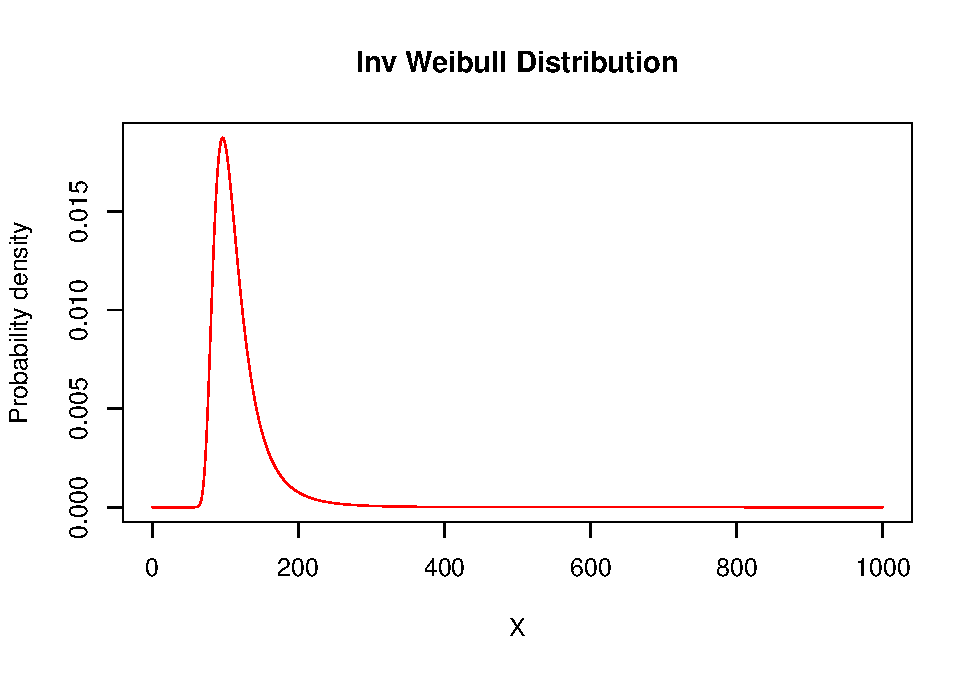
\includegraphics{LDASupplements_files/figure-latex/unnamed-chunk-12-1.pdf}

\[
{\small
\begin{matrix}
\begin{array}{l|c}
\hline
  \text{Density Function} & \text{dinvweibull}(x=, shape=\tau, scale=\theta) \\
\hline
  \text{Distribution Function} & \text{pinvweibull}(p=, shape=\tau,scale=\theta) \\
\hline
  \text{Quantile Function} & \text{qinvweibull}(q=, shape=\tau,scale=\theta) \\ 
\hline
  \text{Random Sampling Function} & \text{rinvweibull}(n=, shape=\tau,scale=\theta) \\
\hline
\end{array}
\end{matrix}
}
\]

\section{One Parameter Distributions}\label{one-parameter-distributions}

Exponential

Inv Exponential

\hypertarget{1pA}{}
{Hide}

Exponential

\[
{\small
\begin{matrix}
\begin{array}{l|c}
\hline
  \text{Name} & \text{Function} \\
\hline
  \text{Parameter Assumptions} & \theta>0 \\
\hline
  \text{Probability Density Function} & \frac{1}{\theta}e^{-x/\theta} \\
    \text{f(x)} & \\
\hline
  \text{Cumulative Distribution Function} & 1-e^{-x/\theta} \\
    \text{F(x)} & \\
\hline
 \textit{k}^{th}~\text{Raw Moment}  & \theta^k\Gamma(k+1) \\
  \mathrm{E}[X^k]  & k>-1 \\
\hline
  VaR_p(x) & -\theta ln(1-p) \\
\hline
  \text{Limited Expected Value} & \theta(1-e^{-x/\theta}) \\
  \mathrm{E}[X\wedge x] & \\
\hline
\end{array}
\end{matrix}
}
\]

\begin{Shaded}
\begin{Highlighting}[]
\NormalTok{theta=}\DecValTok{100}
\NormalTok{X=}\KeywordTok{seq}\NormalTok{(}\DataTypeTok{from=}\DecValTok{0}\NormalTok{,}\DataTypeTok{to=}\DecValTok{1000}\NormalTok{,}\DataTypeTok{by=}\DecValTok{1}\NormalTok{)}
\KeywordTok{plot}\NormalTok{(}\DataTypeTok{x=}\NormalTok{X,}\DataTypeTok{y=}\KeywordTok{dexp}\NormalTok{(X,}\DataTypeTok{rate=}\DecValTok{1}\OperatorTok{/}\NormalTok{theta),}\DataTypeTok{type=}\StringTok{"l"}\NormalTok{,}\DataTypeTok{ylab=}\StringTok{"Probability density"}\NormalTok{,}\DataTypeTok{col=}\StringTok{"red"}\NormalTok{,}\DataTypeTok{main=}\StringTok{"Exponential Distribution"}\NormalTok{)}
\end{Highlighting}
\end{Shaded}

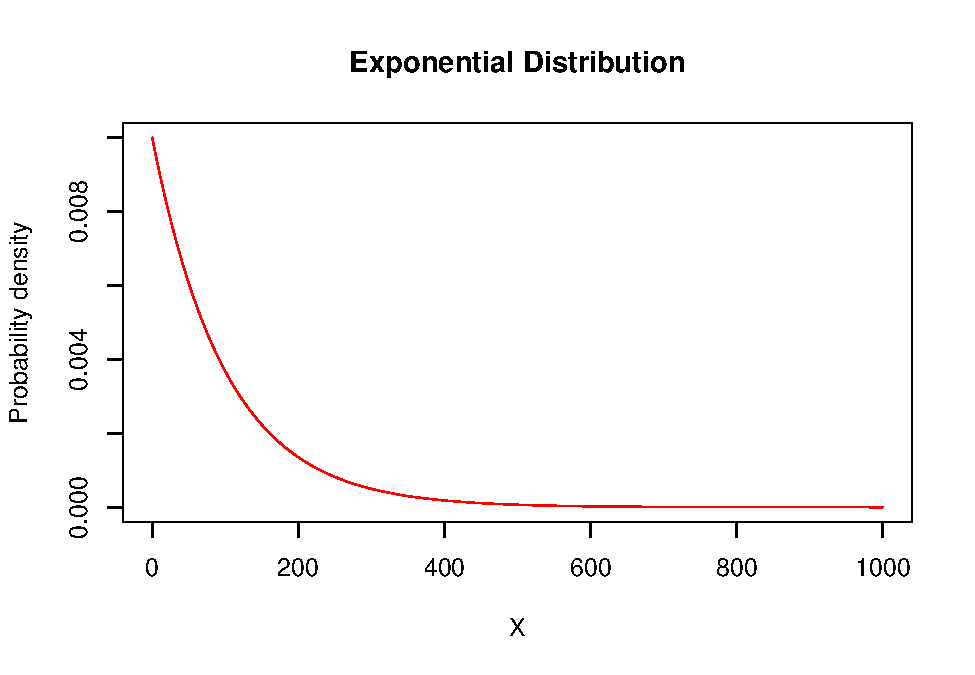
\includegraphics{LDASupplements_files/figure-latex/unnamed-chunk-13-1.pdf}

\[
{\small
\begin{matrix}
\begin{array}{l|c}
\hline
  \text{Density Function} & \text{dexp}(x=, rate=1/\theta) \\
\hline
  \text{Distribution Function} & \text{pexp}(p=, rate=1/\theta) \\
\hline
  \text{Quantile Function} & \text{qexp}(q=, rate=1/\theta) \\ 
\hline
  \text{Random Sampling Function} & \text{rexp}(n=, rate=1/\theta) \\
\hline
\end{array}
\end{matrix}
}
\]

\hypertarget{1pB}{}
{Hide}

Inv Exponential

\[
{\small
\begin{matrix}
\begin{array}{l|c}
\hline
  \text{Name} & \text{Function} \\
\hline
  \text{Probability Density Function} & \frac{\theta e^{-\theta/x}}{x^2} \\
    \text{f(x)} & \\
\hline
  \text{Cumulative Distribution Function} & e^{-\theta/x} \\
    \text{F(x)} & \\
\hline
  \textit{k}^{th}~\text{Raw Moment} & \theta^k\Gamma(k+1) \\
  \mathrm{E}[X^k]  & k>-1 \\
\hline
  \mathrm{E}[(X\wedge x)^k] & \theta^k\Gamma(k+1)\Gamma(k+1;x/\theta)+x^k e^{-x/\theta} \\
  & k>-1 \\
\hline
\end{array}
\end{matrix}
}
\]

\begin{Shaded}
\begin{Highlighting}[]
\NormalTok{theta=}\DecValTok{100}
\NormalTok{X=}\KeywordTok{seq}\NormalTok{(}\DataTypeTok{from=}\DecValTok{0}\NormalTok{,}\DataTypeTok{to=}\DecValTok{1000}\NormalTok{,}\DataTypeTok{by=}\DecValTok{1}\NormalTok{)}
\KeywordTok{plot}\NormalTok{(}\DataTypeTok{x=}\NormalTok{X,}\DataTypeTok{y=}\KeywordTok{dinvexp}\NormalTok{(X,}\DataTypeTok{scale=}\NormalTok{theta),}\DataTypeTok{type=}\StringTok{"l"}\NormalTok{,}\DataTypeTok{ylab=}\StringTok{"Probability density"}\NormalTok{,}\DataTypeTok{col=}\StringTok{"red"}\NormalTok{,}\DataTypeTok{main=}\StringTok{"Inv Exponential Distribution"}\NormalTok{)}
\end{Highlighting}
\end{Shaded}

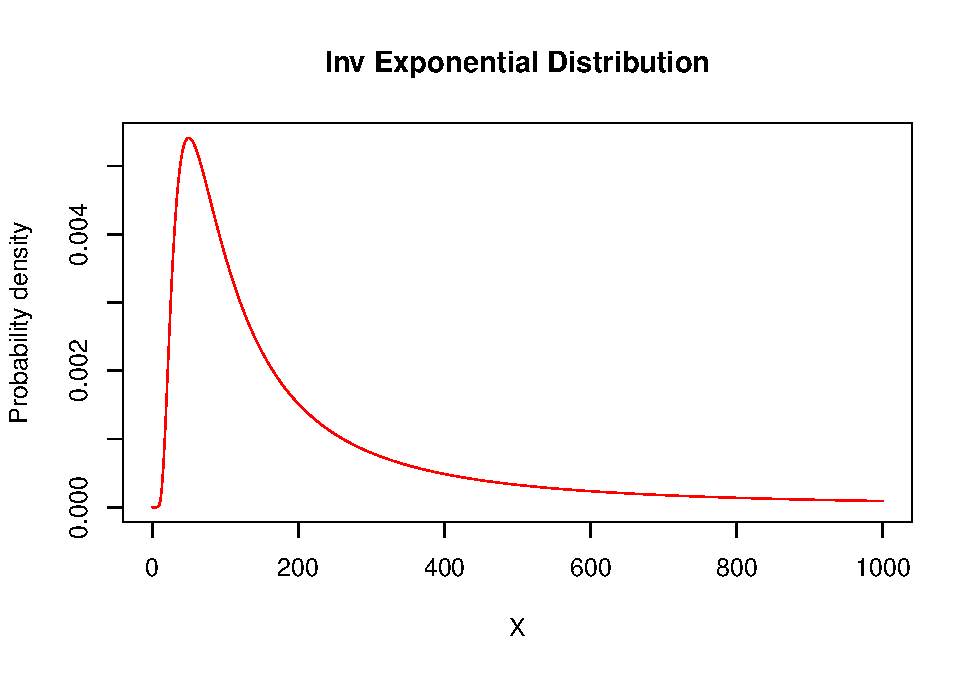
\includegraphics{LDASupplements_files/figure-latex/unnamed-chunk-14-1.pdf}

\[
{\small
\begin{matrix}
\begin{array}{l|c}
\hline
  \text{Density Function} & \text{dinvexp}(x=, scale=\theta) \\
\hline
  \text{Distribution Function} & \text{pinvexp}(p=, scale=\theta) \\
\hline
  \text{Quantile Function} & \text{qinvexp}(q=, scale=\theta) \\ 
\hline
  \text{Random Sampling Function} & \text{rinvexp}(n=, scale=\theta) \\
\hline
\end{array}
\end{matrix}
}
\]

\section{Other distributions}\label{other-distributions}

Lognormal

Inv Gaussian

Single-Parameter Pareto

\hypertarget{odA}{}
{Hide}

Lognormal

\[
{\small
\begin{matrix}
\begin{array}{l|c}
\hline
  \text{Name} & \text{Function} \\
\hline
  \text{Parameter Assumptions} & -\infty <\mu <\infty, \sigma>0 \\
\hline
  \text{Probability Density Function} & \frac{1}{x\sqrt{2\pi}\sigma} \exp\left( -\frac{(\ln x-\mu)^2}{2\sigma^2}\right) \\
    \text{f(x)} & \\
\hline
  \text{Cumulative Distribution Function} & \Phi\left(\frac{ln(x)-\mu}{\sigma}\right) \\
    \text{F(x)} & \\
\hline
  \textit{k}^{th}~\text{Raw Moment} & \exp(k\mu+\frac{k^2\sigma^2}{2}) \\
  \mathrm{E}[X^k]  & k>-a \\
\hline
  \text{Limited Expected Value} & \exp\Big(k\mu+\frac{k^2\sigma^2}{2}\Big)\Phi\Big(\frac{ln(x)-\mu-k\sigma^2}{\sigma}\Big)+x^k\Big[1-\Phi\Big(\frac{ln(x)-\mu}{\sigma}\Big)\Big]  \\
  \mathrm{E}[X\wedge x] & \\
\hline
\end{array}
\end{matrix}
}
\]

\begin{Shaded}
\begin{Highlighting}[]
\NormalTok{dlognorm=}\ControlFlowTok{function}\NormalTok{(x,mu,sigma)\{}
\NormalTok{  p=(}\DecValTok{1}\OperatorTok{/}\NormalTok{(x}\OperatorTok{*}\NormalTok{sigma}\OperatorTok{*}\KeywordTok{sqrt}\NormalTok{(}\DecValTok{2}\OperatorTok{*}\NormalTok{pi)))}\OperatorTok{*}\KeywordTok{exp}\NormalTok{(}\OperatorTok{-}\NormalTok{((}\KeywordTok{log}\NormalTok{(x)}\OperatorTok{-}\NormalTok{mu)}\OperatorTok{/}\NormalTok{sigma)}\OperatorTok{^}\DecValTok{2}\NormalTok{)}
  \KeywordTok{return}\NormalTok{(p)}
\NormalTok{\}}
\end{Highlighting}
\end{Shaded}

\begin{Shaded}
\begin{Highlighting}[]
\NormalTok{mu=}\DecValTok{20}
\NormalTok{sigma=}\DecValTok{12}
\NormalTok{X=}\KeywordTok{seq}\NormalTok{(}\DataTypeTok{from=}\DecValTok{0}\NormalTok{,}\DataTypeTok{to=}\DecValTok{1000}\NormalTok{,}\DataTypeTok{by=}\DecValTok{1}\NormalTok{)}
\KeywordTok{plot}\NormalTok{(}\DataTypeTok{x=}\NormalTok{X,}\DataTypeTok{y=}\KeywordTok{dlognorm}\NormalTok{(X,}\DataTypeTok{mu=}\NormalTok{mu,}\DataTypeTok{sigma=}\NormalTok{sigma),}\DataTypeTok{type=}\StringTok{"l"}\NormalTok{,}\DataTypeTok{col=}\StringTok{"red"}\NormalTok{)}
\end{Highlighting}
\end{Shaded}

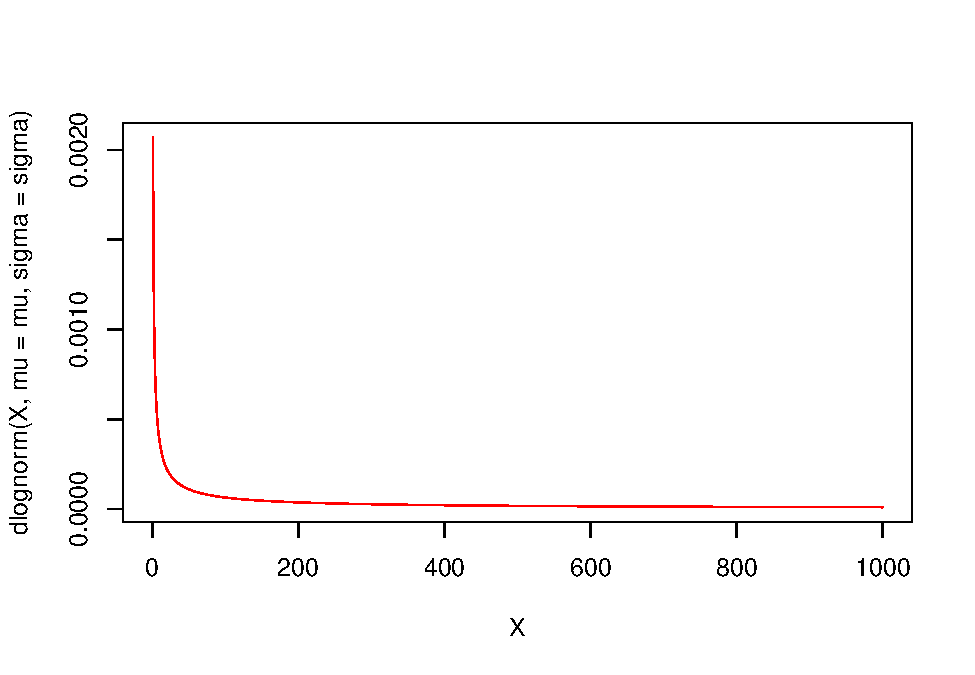
\includegraphics{LDASupplements_files/figure-latex/unnamed-chunk-16-1.pdf}

\hypertarget{odB}{}
{Hide}

Inv Gaussian

\[
{\small
\begin{matrix}
\begin{array}{l|c}
\hline
  \text{Name} & \text{Function} \\
\hline
  \text{Parameter Assumptions} & z=\frac{x-\mu}{\mu}~,~y=\frac{x+\mu}{\mu} \\
\hline
  \text{Probability Density Function} & \Big(\frac{\theta}{2\pi x^3}\Big)^{1/2}\exp\Big(\frac{\theta z^2}{2x}\Big) \\
    \text{f(x)} & \\
\hline
  \text{Cumulative Distribution Function} & \Phi\Big[z\Big(\frac{\theta}{x}\Big)^{1/2}\Big]+\exp\Big(\frac{2\theta}{\mu}\Big)\Phi\Big[-y\Big(\frac{\theta}{x}\Big)^{1/2}\Big] \\
    \text{F(x)} & \\
\hline
  \text{Mean} & \mu \\
  \mathrm{E}[X]  & \\
\hline
  \mathrm{Var[X]} & \frac{\mu^3}{\theta}\\
\hline
  \mathrm{E}[(X\wedge x)^k] & x-\mu x\Phi\Big[z\Big(\frac{\theta}{x}\Big)^{1/2}\Big]-(\mu y)\exp\Big(\frac{2\theta}{\mu}\Big)\Phi\Big[-y\Big(\frac{\theta}{x}\Big)^{1/2}\Big] \\
  &  \\
\hline
\end{array}
\end{matrix}
}
\]

\begin{Shaded}
\begin{Highlighting}[]
\NormalTok{mu=}\DecValTok{100}
\NormalTok{theta=}\DecValTok{1000}
\NormalTok{X=}\KeywordTok{seq}\NormalTok{(}\DataTypeTok{from=}\DecValTok{0}\NormalTok{,}\DataTypeTok{to=}\DecValTok{100}\NormalTok{,}\DataTypeTok{by=}\DecValTok{1}\NormalTok{)}
\KeywordTok{plot}\NormalTok{(}\DataTypeTok{x=}\NormalTok{X,}\DataTypeTok{y=}\KeywordTok{dinvgauss}\NormalTok{(X,}\DataTypeTok{mean=}\NormalTok{mu,}\DataTypeTok{dispersion=}\NormalTok{theta),}\DataTypeTok{type=}\StringTok{"l"}\NormalTok{,}\DataTypeTok{ylab=}\StringTok{"Probability density"}\NormalTok{,}\DataTypeTok{col=}\StringTok{"red"}\NormalTok{,}\DataTypeTok{main=}\StringTok{"Inv Gaussian Distribution"}\NormalTok{)}
\end{Highlighting}
\end{Shaded}

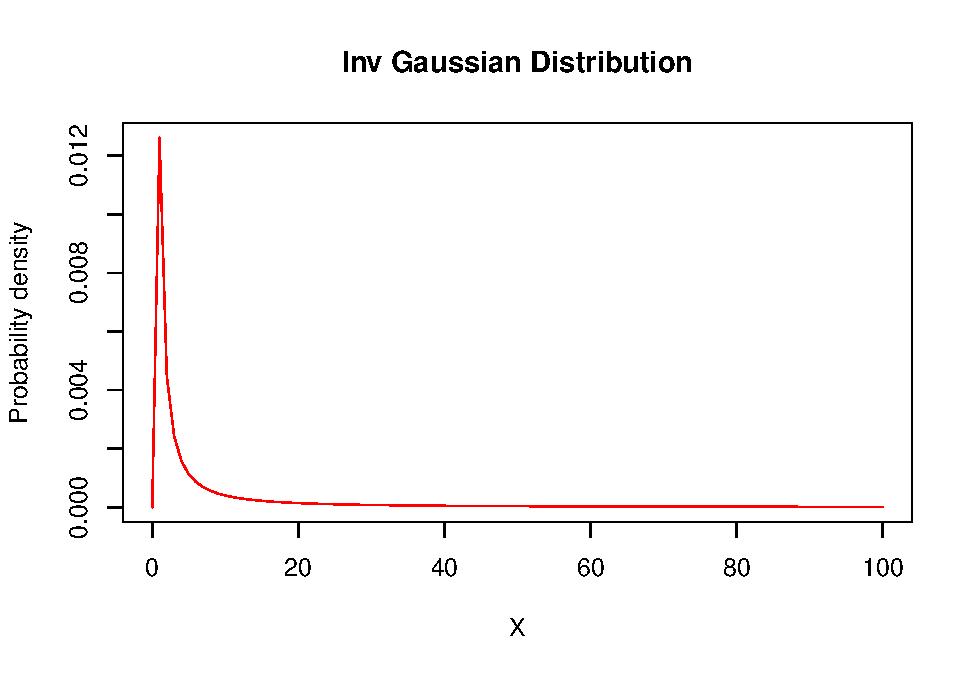
\includegraphics{LDASupplements_files/figure-latex/unnamed-chunk-17-1.pdf}

\[
{\small
\begin{matrix}
\begin{array}{l|c}
\hline
  \text{Density Function} & \text{dinvgauss}(x=, mean=\mu,dispersion=\theta) \\
\hline
  \text{Distribution Function} & \text{pinvgauss}(p=, mean=\mu,dispersion=\theta) \\
\hline
  \text{Quantile Function} & \text{qinvgauss}(q=, mean=\mu,dispersion=\theta) \\ 
\hline
  \text{Random Sampling Function} & \text{rinvgauss}(n=, mean=\mu,dispersion=\theta) \\
\hline
\end{array}
\end{matrix}
}
\]

\hypertarget{odC}{}
{Hide}

Single Parameter Pareto

\[
{\small
\begin{matrix}
\begin{array}{l|c}
\hline
  \text{Name} & \text{Function} \\
\hline
  \text{Parameter Assumptions} & \theta~\text{is known.}~,~x>\theta \\
\hline
  \text{Probability Density Function} & \frac{\alpha\theta^\alpha}{x^{\alpha+1}} \\
    \text{f(x)} & \\
\hline
  \text{Cumulative Distribution Function} & 1-(\theta/x)^\alpha \\
    \text{F(x)} & \\
\hline
  \textit{k}^{th}~\text{Raw Moment} & \frac{\alpha\theta^k}{\alpha-k} \\
  \mathrm{E}[X^k]  & \\
\hline
  \mathrm{E}[(X\wedge x)^k] & \frac{\alpha\theta^k}{\alpha-k}-\frac{k\theta^k}{(\alpha-k)x^{\alpha-k}} \\
  & x \geq\theta \\
\hline
\end{array}
\end{matrix}
}
\]

\begin{Shaded}
\begin{Highlighting}[]
\NormalTok{alpha=}\DecValTok{3}
\NormalTok{theta=}\DecValTok{100}
\NormalTok{X=}\KeywordTok{seq}\NormalTok{(}\DataTypeTok{from=}\DecValTok{0}\NormalTok{,}\DataTypeTok{to=}\DecValTok{1000}\NormalTok{,}\DataTypeTok{by=}\DecValTok{1}\NormalTok{)}
\KeywordTok{plot}\NormalTok{(}\DataTypeTok{x=}\NormalTok{X,}\DataTypeTok{y=}\KeywordTok{dpareto1}\NormalTok{(X,}\DataTypeTok{shape=}\NormalTok{alpha,}\DataTypeTok{min=}\NormalTok{theta),}\DataTypeTok{type=}\StringTok{"l"}\NormalTok{,}\DataTypeTok{ylab=}\StringTok{"Probability density"}\NormalTok{,}\DataTypeTok{col=}\StringTok{"red"}\NormalTok{,}\DataTypeTok{main=}\StringTok{"Single Parameter Pareto Distribution"}\NormalTok{)}
\end{Highlighting}
\end{Shaded}

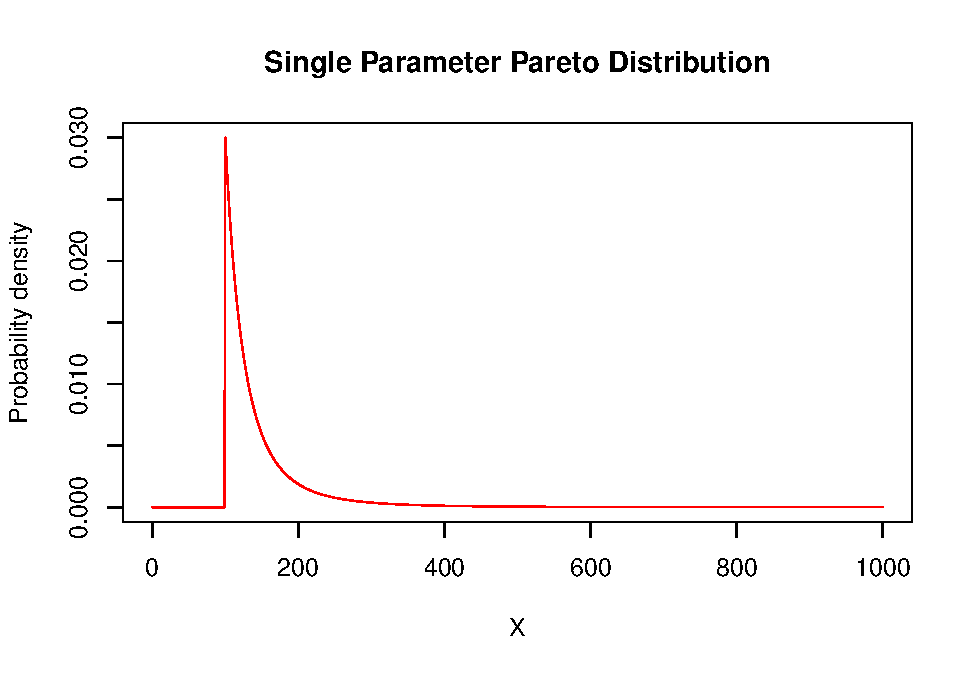
\includegraphics{LDASupplements_files/figure-latex/unnamed-chunk-18-1.pdf}

\[
{\small
\begin{matrix}
\begin{array}{l|c}
\hline
  \text{Density Function} & \text{dpareto1}(x=, shape=\alpha,min=\theta) \\
\hline
  \text{Distribution Function} & \text{ppareto1}(p=, shape=\alpha,min=\theta) \\
\hline
  \text{Quantile Function} & \text{qpareto1}(q=, shape=\alpha,min=\theta) \\ 
\hline
  \text{Random Sampling Function} & \text{rpareto1}(n=, shape=\alpha,min=\theta) \\
\hline
\end{array}
\end{matrix}
}
\]

\section{Distributions with Finite
Support}\label{distributions-with-finite-support}

General Beta

Beta

\hypertarget{fsA}{}
{Hide}

Generalized Beta

\[
{\small
\begin{matrix}
\begin{array}{l|c}
\hline
  \text{Name} & \text{Function} \\
\hline
  \text{Parameter Assumptions} & 0<x<\theta~,~u=(x/\theta)^\tau \\
\hline
  \text{Probability Density Function} & \frac{\Gamma(a+b)}{\Gamma(a)\Gamma(b)}u^\alpha(1-u)^{b-1}\frac{\tau}{x} \\
    \text{f(x)} & \\
\hline
  \text{Cumulative Distribution Function} & \beta(a,b;u) \\
    \text{F(x)} & \\
\hline
  \textit{k}^{th}~\text{Raw Moment} & \frac{\theta^k\Gamma(a+b)\Gamma(a+(k/\tau))}{\Gamma(a)\Gamma(a+b+(k/\tau))} \\
   \mathrm{E}[X^k] & k>-\alpha\tau \\
\hline
  \mathrm{E}[(X\wedge x)^k] & \frac{\theta^k\Gamma(a+b)\Gamma(a+(k/\tau))}{\Gamma(a)\Gamma(a+b+(k/\tau))}\beta(a+(k/\tau),b;u)+x^k[1-\beta(a,b;u)] \\
\hline
\end{array}
\end{matrix}
}
\]

\begin{Shaded}
\begin{Highlighting}[]
\NormalTok{a=}\DecValTok{3}
\NormalTok{b=}\DecValTok{5}
\NormalTok{tau=}\DecValTok{2}
\NormalTok{theta=}\DecValTok{1000}
\NormalTok{X=}\KeywordTok{seq}\NormalTok{(}\DataTypeTok{from=}\DecValTok{0}\NormalTok{,}\DataTypeTok{to=}\DecValTok{1000}\NormalTok{,}\DataTypeTok{by=}\DecValTok{1}\NormalTok{)}
\KeywordTok{plot}\NormalTok{(}\DataTypeTok{x=}\NormalTok{X,}\DataTypeTok{y=}\KeywordTok{dgenbeta}\NormalTok{(X,}\DataTypeTok{shape1=}\NormalTok{a,}\DataTypeTok{shape2=}\NormalTok{b,}\DataTypeTok{shape3=}\NormalTok{tau,}\DataTypeTok{scale=}\NormalTok{theta),}\DataTypeTok{type=}\StringTok{"l"}\NormalTok{,}\DataTypeTok{ylab=}\StringTok{"Probability density"}\NormalTok{,}\DataTypeTok{col=}\StringTok{"red"}\NormalTok{,}\DataTypeTok{main=}\StringTok{"Generalized Beta Distribution"}\NormalTok{)}
\end{Highlighting}
\end{Shaded}

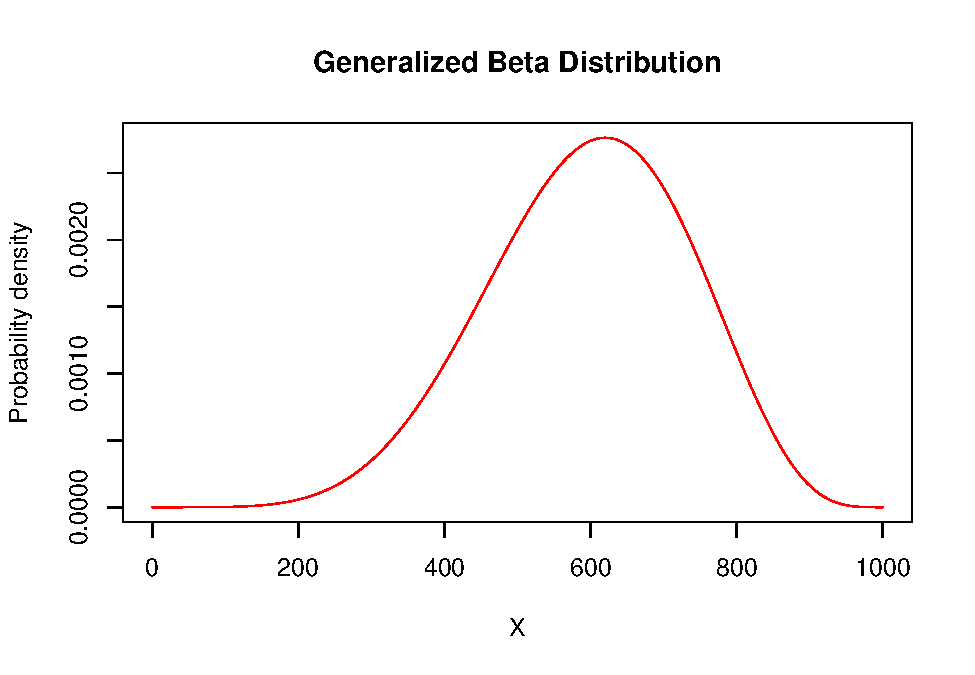
\includegraphics{LDASupplements_files/figure-latex/unnamed-chunk-19-1.pdf}

\[
{\small
\begin{matrix}
\begin{array}{l|c}
\hline
  \text{Density Function} & \text{dgenbeta}(x=, shape1=a,shape2=b,shape3=\tau,scale=\theta) \\
\hline
  \text{Distribution Function} & \text{pgenbeta}(p=, shape1=a,shape2=b,shape3=\tau,scale=\theta) \\
\hline
  \text{Quantile Function} & \text{qgenbeta}(q=, shape1=a,shape2=b,shape3=\tau,scale=\theta) \\ 
\hline
  \text{Random Sampling Function} & \text{rgenbeta}(n=, shape1=a,shape2=b,shape3=\tau,scale=\theta) \\
\hline
\end{array}
\end{matrix}
}
\]

\hypertarget{fsB}{}
{Hide}

Beta

\[
{\small
\begin{matrix}
\begin{array}{l|c}
\hline
  \text{Name} & \text{Function} \\
\hline
  \text{Parameter Assumptions} & u=\frac{x}{\theta},~a>0,~b>0,~0<x<\theta \\
\hline
  \text{Probability Density Function} & \frac{\Gamma(a+b)}{\Gamma(a)\Gamma(b)} u^a(1-u)^{b-1}\frac{1}{x} \\
    \text{f(x)} & \\
\hline
  \text{Cumulative Distribution Function} & \beta(a,b;u) \\
    \text{F(x)} & \\
\hline
  \textit{k}^{th}~\text{Raw Moment} & \frac{\theta^k 
  \Gamma(a+b)\Gamma(a+k)}{\Gamma(a)\Gamma(a+b+1)} \\
  \mathrm{E}[X^k]  & k>-a \\
\hline
  \text{Limited Expected Value} & \frac{\theta^k a(a+1)\cdots(a+k-1)}{(a+b)(a+b+1)\cdots(a+b+k-1)}\beta(a+k,b;u)+x^k[1-\beta(a,b;u)]  \\
   \mathrm{E}[X\wedge x] & k > -\alpha \\
\hline
\end{array}
\end{matrix}
}
\]

\begin{Shaded}
\begin{Highlighting}[]
\NormalTok{a=}\DecValTok{2}
\NormalTok{b=}\DecValTok{4}
\NormalTok{theta=}\DecValTok{1}
\NormalTok{X=}\KeywordTok{seq}\NormalTok{(}\DataTypeTok{from=}\DecValTok{0}\NormalTok{,}\DataTypeTok{to=}\DecValTok{1}\NormalTok{,}\DataTypeTok{by=}\NormalTok{.}\DecValTok{0001}\NormalTok{)}
\KeywordTok{plot}\NormalTok{(}\DataTypeTok{x=}\NormalTok{X,}\DataTypeTok{y=}\KeywordTok{dbeta}\NormalTok{(X,}\DataTypeTok{shape1=}\NormalTok{a,}\DataTypeTok{shape2=}\NormalTok{b,}\DataTypeTok{ncp=}\NormalTok{theta),}\DataTypeTok{type=}\StringTok{"l"}\NormalTok{,}\DataTypeTok{ylab=}\StringTok{"Probability density"}\NormalTok{,}\DataTypeTok{col=}\StringTok{"red"}\NormalTok{,}\DataTypeTok{main=}\StringTok{"Beta Distribution"}\NormalTok{)}
\end{Highlighting}
\end{Shaded}

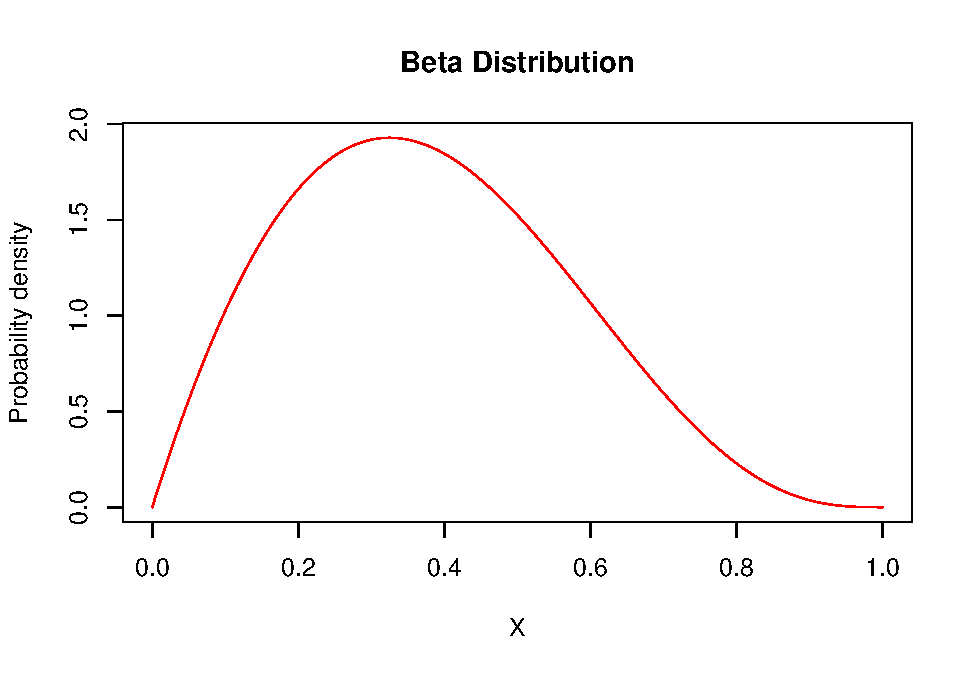
\includegraphics{LDASupplements_files/figure-latex/unnamed-chunk-20-1.pdf}

\[
{\small
\begin{matrix}
\begin{array}{l|c}
\hline
  \text{Density Function} & \text{dbeta}(x=, shape1=a,shape2=b,ncp=\theta) \\
\hline
  \text{Distribution Function} & \text{pbeta}(p=, shape1=a,shape2=b,ncp=\theta) \\
\hline
  \text{Quantile Function} & \text{qbeta}(q=, shape1=a,shape2=b,ncp=\theta) \\ 
\hline
  \text{Random Sampling Function} & \text{rbeta}(n=, shape1=a,shape2=b,ncp=\theta) \\
\hline
\end{array}
\end{matrix}
}
\]

\section{Limited Expected Values}\label{limited-expected-values}

Functions

Graph

\hypertarget{levA}{}
{Hide}

Functions

\[
{\small
\begin{matrix}
\begin{array}{l|c}
\hline
  \text{Distribuion} & \text{Function} \\
\hline
  \text{GB2} & 
  \frac{\theta\Gamma(\tau+1)\Gamma(\alpha-1)}{\Gamma(\alpha)\Gamma(\tau)}\beta(\tau+1,\alpha-1;\frac{x}{x+\beta})+x[1-\beta(\tau,\alpha;\frac{x}{x+\beta})] \\
\hline
  \text{Burr} & \frac{\theta\Gamma(1+\frac{1}{\tau})\Gamma(\alpha-\frac{1}{\gamma})}{\Gamma(\alpha)}\beta(1+\frac{1}{\gamma},\alpha-\frac{1}{\gamma};1-\frac{1}{1+(x/\theta)^\gamma})+x\Big(\frac{1}{1+(x/\theta)^\gamma}\Big)^\alpha \\
\hline
  \text{Inverse Burr} & \frac{\theta\Gamma(1+(1/\gamma))\Gamma(1-(1/\gamma))}{\Gamma(\gamma)}\beta(\tau+\frac{1}{\gamma},1-\frac{1}{\gamma};\frac{(x/\theta)^\gamma}{1+(x/\theta)^\gamma})+x[1-\Big(\frac{(x/\theta)^\gamma}{1+(x/\theta)^\gamma}\Big)^\tau] \\
\hline
  \text{Pareto} & \\
  \alpha=1 & -\theta ln\Big(\frac{\theta}{x+\theta}\Big) \\
  \alpha\neq1 & \frac{\theta}{\alpha-1}[1-\Big(\frac{\theta}{x+\theta}\Big)^{\alpha-1}] \\
\hline
  \text{Inverse Pareto} & \theta\tau\int^{x/(x+\theta)}_0~y^\tau(1-y)^{-1}dy+x[1-\Big(\frac{x}{x+\theta}\Big)^\tau] \\
\hline
  \text{Logistic} & \theta\Gamma_1(1+\frac{1}{\gamma})\Gamma(1-\frac{1}{\gamma})\beta(1+\frac{1}{\gamma},1-\frac{1}{\gamma};\frac{(x/\theta)^\gamma}{1+(x/\theta)^\gamma})+x(1-\frac{(x/\theta)^\gamma}{1+(x/\theta)^\gamma})  \\
\hline
  \text{Paralogistic} & \frac{\theta\Gamma(1+\frac{1}{\alpha})\Gamma(\alpha-\frac{1}{\alpha})}{\Gamma(\alpha)}\beta(1+\frac{1}{\alpha},\alpha-\frac{1}{\alpha};1-\frac{1}{1+(x/\theta)^\alpha})+x\Big(\frac{1}{1+(x/\theta)^\alpha}\Big)^\alpha \\
\hline
  \text{Inverse Paralogistic} & \frac{\theta\Gamma(\tau+\frac{1}{\tau})\Gamma(1-\frac{1}{\tau})}{\Gamma(\tau)}\beta(\tau+\frac{1}{\tau},1-\frac{1}{\tau};\frac{(x/\theta)^\tau}{1+(x/\theta)^\tau})+x[1-\Big(\frac{(x/\theta)^\tau}{1+(x/\theta)^\tau}\Big)^\tau] \\
\hline
  \text{Gamma} & \frac{\theta\Gamma(\alpha+1)}{\Gamma(\alpha)}\Gamma(\alpha+k;\frac{x}{\theta})+x[1-\Gamma(\alpha,\frac{x}{\theta})] \\
\hline
  \text{Inverse Gamma} & \frac{\theta\Gamma(\alpha-1)}{\Gamma(\alpha)}[1-\Gamma(\alpha-1;\frac{\theta}{x})]+x\Gamma(\alpha,\frac{\theta}{x}) \\
\hline
  \text{Weibull} & \theta\Gamma(1+\frac{1}{\tau})\Gamma(1+\frac{1}{\tau},\Big(\frac{x}{\theta}\Big)^\tau)+x*\exp(-(x/\theta)^\tau) \\
\hline
  \text{Inverse Weibull} & \theta\Gamma(1-\frac{1}{\tau})[1-\Gamma(1-\frac{1}{\tau};\Big(\frac{\theta}{x}\Big)^\tau)]+x[1-\exp(-(\theta/x)^\tau)] \\
\hline
  \text{Exponential} & \theta(1-\exp(-(x/\theta))) \\
\hline
  \text{Inverse Exponential} & \theta G(0;\frac{\theta}{x})+x(1-\exp(-(\theta/x))) \\
\hline
  \text{Lognormal} & \exp(\mu+\sigma^2/2)\Phi\Big(\frac{ln(x)-\mu-\sigma^2}{\sigma}\Big)+x[1-\Phi\Big(\frac{ln(x)-\mu}{\sigma}\Big)] \\
\hline
  \text{Inverse Gaussian} & x-\mu\Big(\frac{x-\mu}{\mu}\Big)\Phi\Big[\Big(\frac{x-\mu}{\mu}\Big)\Big(\frac{\theta}{x}\Big)^{1/2}\Big]-\mu\Big(\frac{x+\mu}{\mu}\Big)\exp\Big(\frac{2\theta}{\mu}\Big)\Phi\Big[-\Big(\frac{x+\mu}{\mu}\Big)\Big(\frac{\theta}{x}\Big)^{1/2}\Big] \\
\hline
  \text{Single-Parameter Pareto} & \frac{\alpha\theta}{\alpha-1}-\frac{\theta^\alpha}{(\alpha-1)x^{\alpha-1}} \\
\hline
  \text{Generalized Beta} & \frac{\theta\Gamma(a+b)\Gamma(a+\frac{1}{\tau})}{\Gamma(a)\Gamma(a+b+\frac{1}{\tau})}\beta(a+\frac{1}{\tau},b;\Big(\frac{x}{\theta}\Big)^\tau)+x\Big[1-\beta(a,b;\Big(\frac{x}{\theta}\Big)^\tau)\Big] \\
\hline
  \text{Beta} & \frac{\theta a}{(a+b)}\beta(a+1,b;\frac{x}{\theta})+x[1-\beta(a,b;\frac{x}{\theta})] \\
\hline
\end{array}
\end{matrix}
}
\]

\hypertarget{levB}{}
{Hide}

Graphs

\[
{\small
\begin{matrix}
\begin{array}{l|c|c}
\hline
  \text{Distribution} & \text{Parameters} & \mathrm{E}[x] & E[X\wedge100] & E[X\wedge250] & E[X\wedge500] &E[X\wedge1000] \\
\hline
  \text{Pareto} & \alpha=3, \theta=200 & 100 & 55.55 &80.25 & 91.84 & 97.22  \\ 
\hline
  \text{Exponential} & \theta=100 & 100 & 63.21 & 91.79 & 99.33 & 99.99 \\
\hline
  \text{Gamma} & \alpha=2, \theta=50 & 100 & 72.93 & 97.64 & 99.97 & 100 \\
\hline
  \text{Weibull} & \tau=2, \theta=\frac{200}{\sqrt[]{\pi}} & 100 & 78.99 & 99.82 & 100 & 100 \\
\hline
  \text{GB2} & \alpha=3,\tau=2,\theta=100 & 100 & 62.50 & 86.00 & 94.91 & 98.42  \\
\hline
\end{array}
\end{matrix}
}
\]

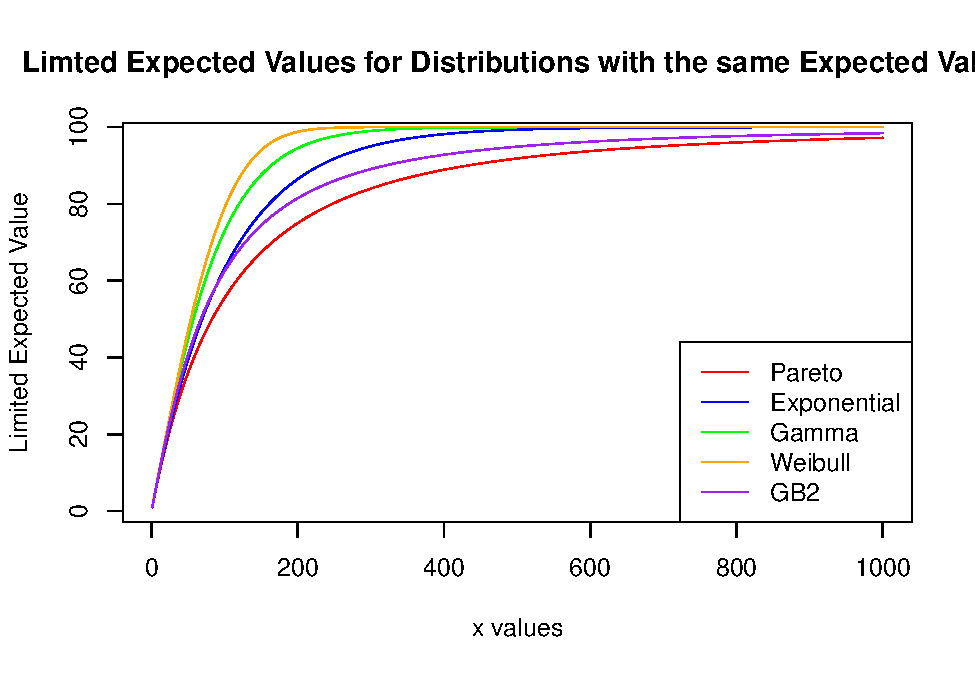
\includegraphics{LDASupplements_files/figure-latex/unnamed-chunk-22-1.pdf}

\chapter{Discrete Distributions}\label{discrete-distributions}

\textbf{Chapter Preview}.

This table of distributions is a summary of selected discrete
probability distributions used throughout \emph{Loss Data Analytics}.

\section{(a,b,0) Class Distributions}\label{ab0-class-distributions}

Poisson

Geometric

Binomial

Negative Binomial

\hypertarget{disA}{}
{Hide}

Poisson

\[
{\small
\begin{matrix}
\begin{array}{l|c}
\hline
  \text{Name} & \text{Function} \\
\hline
  p_0 & e^{-\lambda} \\
\hline
  \text{Probability Mass Function} & \frac{e^{-\lambda}\lambda^k}{k!} \\
  p_k & \\
\hline
  \text{Expected Value} & \lambda \\
  \mathrm{E[N]} & \\
\hline
  \text{Variance} & \lambda \\
\hline
  \text{Probability Generating Function} & e^{\lambda(z-1)} \\
  \mathrm{P(z)} & \\
  \hline
  \text{a and b for recursion} & a=0 \\
   & b=\lambda \\
\hline
\end{array}
\end{matrix}
}
\]

\hypertarget{disB}{}
{Hide}

Geometric

\[
{\small
\begin{matrix}
\begin{array}{l|c}
\hline
  \text{Name} & \text{Function} \\
\hline
  p_0 & \frac{1}{1+\beta} \\
\hline
  \text{Probability Mass Function} & \frac{\beta^k}{(1+\beta)^{k+1}} \\
  p_k & \\
\hline
  \text{Expected Value} & \beta \\
  \mathrm{E[N]} & \\
\hline
  \text{Variance} & \beta(1+\beta) \\
\hline
  \text{Probability Generating Function} & [1-\beta(z-1)]^{-1} \\
  \mathrm{P(z)} & \\
  \hline
  \text{a and b for recursion} & a=\frac{\beta}{1+\beta} \\
   & b=0 \\
\hline
\end{array}
\end{matrix}
}
\]

\hypertarget{disC}{}
{Hide}

Binomial

\[
{\small
\begin{matrix}
\begin{array}{l|c}
\hline
  \text{Name} & \text{Function} \\
\hline
  \text{Parameter Assumptions} & 0<q<1,~\text{m is an integer} \\
   & 0 \leq k \leq m\\
\hline
  p_0 &(1-q)^m \\
\hline
  \text{Probability Mass Function} & \binom{m}{k}q^k(1-q)^{m-k} \\
  p_k & \\
\hline
  \text{Expected Value} & mq \\
  \mathrm{E[N]} & \\
\hline
  \text{Variance} & mq(1-q) \\
\hline
  \text{Probability Generating Function} & [1+q(z-1)]^m \\
  \mathrm{P(z)} & \\
  \hline
  \text{a and b for recursion} & a=\frac{-q}{1-q} \\
   & b=\frac{(m+1)q}{1-q} \\
\hline
\end{array}
\end{matrix}
}
\]

\hypertarget{disD}{}
{Hide}

Negative Binomial

\[
{\small
\begin{matrix}
\begin{array}{l|c}
\hline
  \text{Name} & \text{Function} \\
\hline
  p_0 & (1+\beta)^{-r} \\
\hline
  \text{Probability Mass Function} & \frac{r(r+1)\cdots(r+k-1)\beta^k}{k!(1+\beta)^{r+k}} \\
  p_k & \\
\hline
  \text{Expected Value} & r\beta \\
  \mathrm{E[N]} & \\
\hline
  \text{Variance} & r\beta(1+\beta) \\
\hline
  \text{Probability Generating Function} & [1-\beta(z-1)]^{-r} \\
  \mathrm{P(z)} & \\
  \hline
  \text{a and b for recursion} & a=\frac{\beta}{1+\beta} \\
   & b=\frac{(r-1)\beta}{1+\beta} \\
\hline
\end{array}
\end{matrix}
}
\]

\section{(a,b,1) Class Distributions - Zero
Truncated}\label{ab1-class-distributions---zero-truncated}

Zero Truncated Poisson

Zero Truncated Geometric

Zero Truncated Binomial

Zero Truncated Negative Binomial

Logarithmic

\hypertarget{ztA}{}
{Hide}

Zero Truncated Poisson

\[
{\small
\begin{matrix}
\begin{array}{l|c}
\hline
  \text{Name} & \text{Function} \\
\hline
  p^T_1 & \frac{\lambda}{e^\lambda-1} \\
\hline
  \text{Probability Mass Function} & \frac{\lambda^k}{k!(e^\lambda-1)} \\
  p^T_k & \\
\hline
  \text{Expected Value} & \frac{\lambda}{1-e^{-\lambda}} \\
  \mathrm{E[N]} & \\
\hline
  \text{Variance} & \frac{\lambda[1-(\lambda+1)e^{-\lambda}]}{(1-e^{-\lambda})^2} \\
\hline
  \tilde\lambda & ln(\frac{n\hat\mu}{n_1}) \\
\hline
  \text{Probability Generating Function} & \frac{e^{\lambda z}-1}{e^\lambda-1} \\
  \mathrm{P(z)} & \\
\hline
  \text{a and b for recursion} & a=0 \\
   & b=\lambda \\
\hline
\end{array}
\end{matrix}
}
\]

\hypertarget{ztB}{}
{Hide}

Zero Truncated Geometric

\[
{\small
\begin{matrix}
\begin{array}{l|c}
\hline
  \text{Name} & \text{Function} \\
\hline
  p^T_1 & \frac{1}{1+\beta} \\
\hline
  \text{Probability Mass Function} & \frac{\beta^{k-1}}{(1+\beta)^k} \\
  p^T_k & \\
\hline
  \text{Expected Value} & 1+\beta \\
  \mathrm{E[N]} & \\
\hline
  \text{Variance} & \beta(1+\beta) \\
\hline
  \tilde\beta & \hat\mu-1 \\
\hline
  \text{Probability Generating Function} & \frac{[1-\beta(z-1)]^{-1}-(1+\beta)^{-1}}{1-(1+\beta)^{-1}} \\
  \mathrm{P(z)} & \\
\hline
  \text{a and b for recursion} & a=\frac{\beta}{1+\beta} \\
   & b=0 \\
\hline
\end{array}
\end{matrix}
}
\]

\hypertarget{ztC}{}
{Hide}

Zero Truncated Binomial

\[
{\small
\begin{matrix}
\begin{array}{l|c}
\hline
  \text{Name} & \text{Function} \\
\hline
  \text{Parameter Assumptions} & 0<q<1,~\text{m is an integer} \\
   & 0 \leq k \leq m\\
\hline
  p^T_1 & \frac{m(1-q)^{m-1}q}{1-(1-q)^m} \\
\hline
  \text{Probability Mass Function} & \frac{\binom{m}{k}q^k(1-q)^{m-k}}{1-(1-q)^m} \\
  p^T_k & \\
\hline
  \text{Expected Value} & \frac{mq}{1-(1-q)^m} \\
  \mathrm{E[N]} & \\
\hline
  \text{Variance} & \frac{mq[(1-q)-(1-q+mq)(1-q)^m]}{[1-(1-q)^m]^2} \\
\hline
  \tilde q & \frac{\hat\mu}{m} \\
\hline
  \text{Probability Generating Function} & \frac{[1+q(z-1)^m]-(1-q)^m}{1-(1-q)^m} \\
  \mathrm{P(z)} & \\
\hline
  \text{a and b for recursion} & a=\frac{1}{1-q} \\
   & b=\frac{(m+1)q}{1-q} \\
\hline
\end{array}
\end{matrix}
}
\]

\hypertarget{ztD}{}
{Hide}

Zero Truncated Negative Binomial

\[
{\small
\begin{matrix}
\begin{array}{l|c}
\hline
  \text{Name} & \text{Function} \\
\hline
  \text{Parameter Assumptions} & r>-1, r\neq0 \\
\hline
  p^T_1 & \frac{r\beta}{(1+\beta)^{r+1}-(1+\beta)} \\
\hline
  \text{Probability Mass Function} & \frac{r(r+1)\cdots(r+k-1)}{k![(1+\beta)^r-1]}(\frac{\beta}{1+\beta})^k \\
  p^T_k & \\
\hline
  \text{Expected Value} & \frac{r\beta}{1-(1+\beta)^{-r}} \\
  \mathrm{E[N]} & \\
\hline
  \text{Variance} & \frac{r\beta[(1+\beta)-(1+\beta+r\beta)(1+\beta)^{-r}]}{[1-(1+\beta)^{-r}]^2} \\
\hline
  \tilde\beta & \frac{\hat\sigma^2}{\hat\mu}-1 \\
\hline
  \tilde r & \frac{\hat\mu^2}{\hat\sigma^2-\hat\mu} \\
\hline
  \text{Probability Generating Function} & \frac{[1-\beta(z-1)]^{-r}-(1+\beta)^{-r}}{1-(1+\beta)^{-r}} \\
  \mathrm{P(z)} & \\
\hline
  \text{a and b for recursion} & a=\frac{\beta}{1+\beta} \\
   & b=\frac{(r-1)\beta}{1+\beta} \\
\hline
\end{array}
\end{matrix}
}
\]

\hypertarget{ztE}{}
{Hide}

Logarithmic

\[
{\small
\begin{matrix}
\begin{array}{l|c}
\hline
  \text{Name} & \text{Function} \\
\hline
  p^T_1 & \frac{\beta}{(1+\beta)ln(1+\beta)} \\
\hline
  \text{Probability Mass Function} & \frac{\beta^k}{k(1+\beta)^k ln(1+\beta)} \\
  p^T_k & \\
\hline
  \text{Expected Value} & \frac{\beta}{ln(1+\beta)} \\
  \mathrm{E[N]} & \\
\hline
  \text{Variance} & \frac{\beta[1+\beta-\frac{\beta}{ln(1+\beta)}]}{ln(1+\beta)} \\
\hline
  \tilde\beta & \frac{n\hat\mu}{n_1}-1~=~ \frac{2(\hat\mu-1)}{\hat\mu} \\
\hline
  \text{Probability Generating Function} & 1-\frac{ln[1-\beta(z-1)]}{ln(1+\beta)} \\
  \mathrm{P(z)} & \\
\hline
  \text{a and b for recursion} & a=\frac{\beta}{1+\beta} \\
   & b=\frac{-\beta}{1+\beta} \\
\hline
\end{array}
\end{matrix}
}
\]

\bibliography{book.bib,packages.bib}


\end{document}
